%We use \beetle{} and baseline language model surprisals to predict first-pass duration, which reflects []... and is often ...]



% enables us to manipulate model training in ways that may correspond to different kinds of language exposure patterns. At a high level, 


%Psycholinguistic evaluation provides a complementary test of bilingual language models beyond downstream NLP accuracy. Prior work has shown that LM surprisal predicts human reading behaviour across languages and modalities \citep{de-varda-marelli-2023-scaling, wilcox2023language, xu2023linearity}, including L2 reading \citep{de-varda-marelli-2022-effects}. 

% We evaluate whether bilingual exposure curricula alter the alignment between \beetle{} surprisal and human L2 reading times using the metric and mixed-effects specification in App.~\ref{sec:meco-results} (Eq.~\ref{eq:meco-spec}).

% \begin{figure}[t]
%   \centering
%   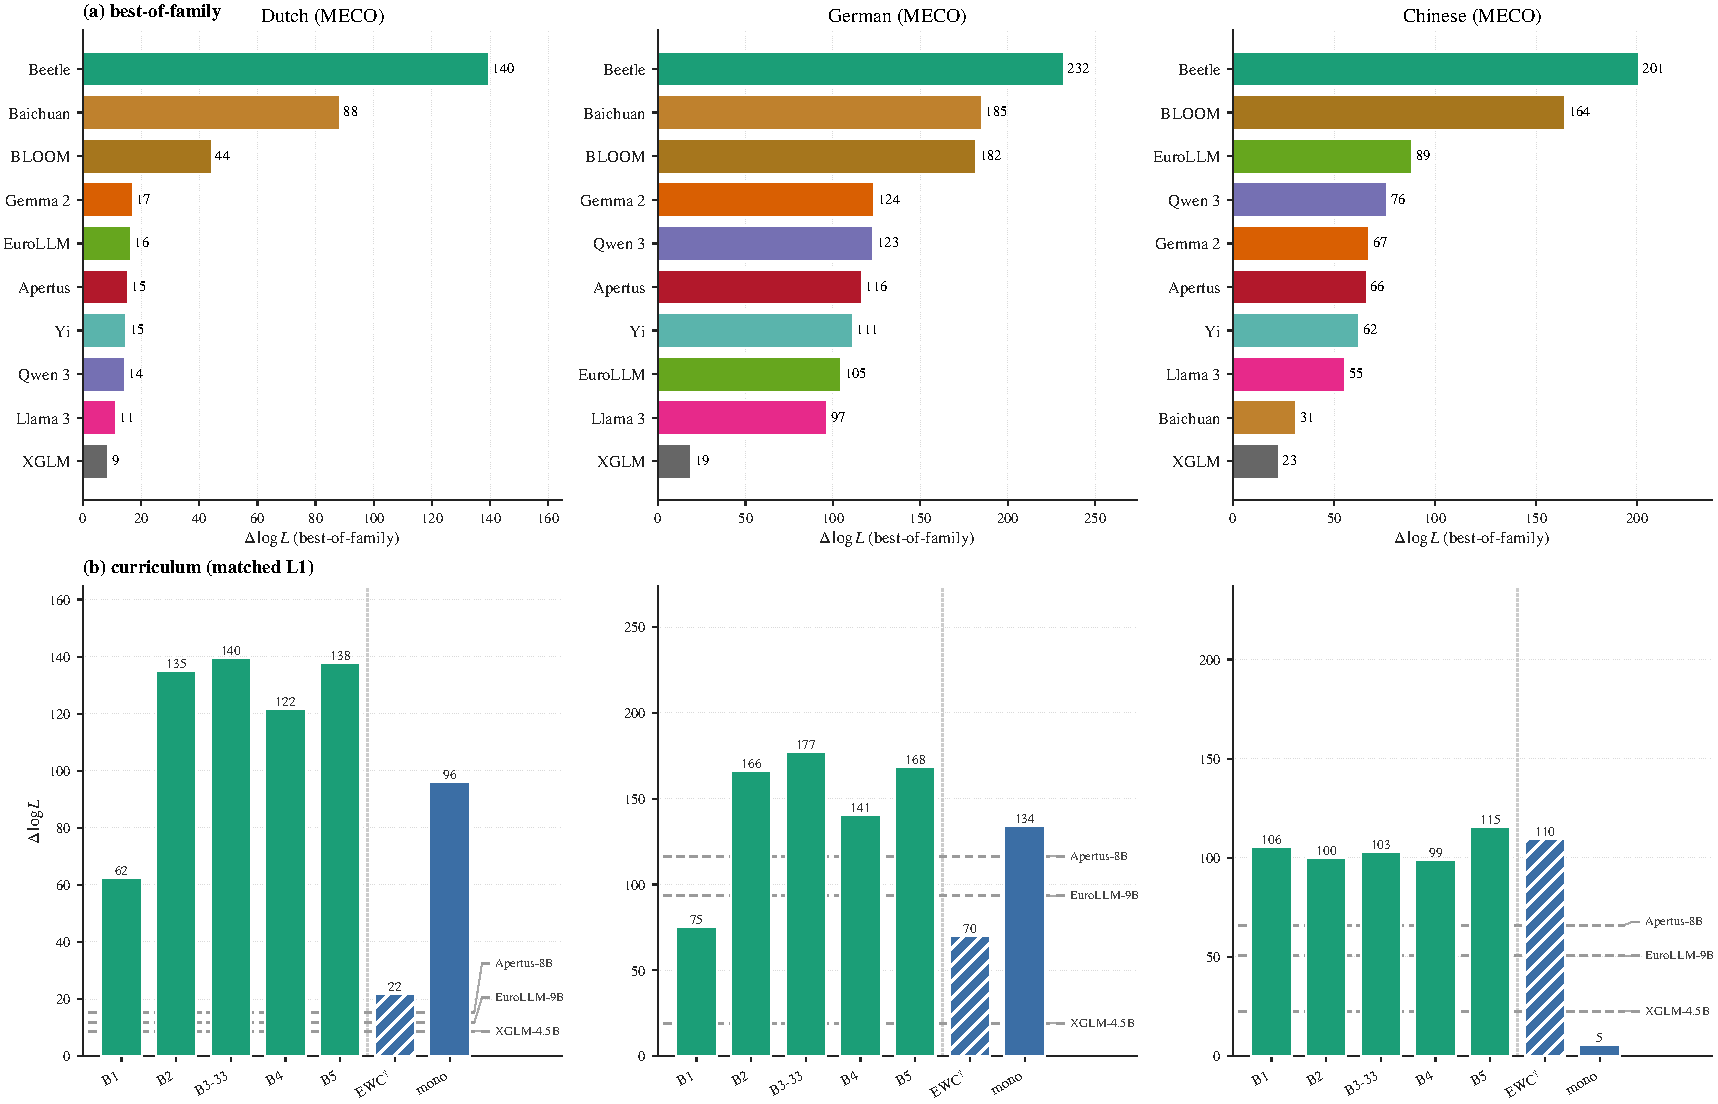
\includegraphics[width=\linewidth]{fig/F3_meco_best_of_family_v2.pdf}
%   \caption{MECO L2 reading-time alignment ($\Delta\log L$) for \beetle{} bilinguals against multilingual baselines. \textbf{(a)}~Best-of-family per-cohort comparison across Dutch, German, and Chinese L1 readers. \textbf{(b)}~\beetle{} curricula (B1--B5) against the EWC bilingual baseline of \citet{constantinescu2025investigating} ($\dagger$) and per-L1 monolingual anchors (bars), with LLM reference levels (XGLM-4.5B, EuroLLM-9B, Apertus-8B) as dashed lines. Higher $\Delta\log L$ = better surprisal--reading-time alignment. Single-seed point estimates; full per-condition results in App.~\ref{sec:meco-results}.}
%   \label{fig:meco_two_col_layout}
% \end{figure}




% %\begin{figure*}[t]
% %  \centering

% %  % ================= LEFT COLUMN =================
%  % \begin{minipage}[t]{0.62\linewidth}
%   %  \centering

%    % \begin{subfigure}[t]{\linewidth}
%     %  \centering
%      % \includegraphics[width=\linewidth]%
%       %  {fig/fig_meco_best_of_family.pdf}
% %    \end{subfigure}

%  %   \vspace{-0.3em}

%  %   \begin{subfigure}[t]{\linewidth}
%  %     \centering
%  %     \includegraphics[width=\linewidth]%
%  %       {fig/meco/F4_curriculum_meco_deltaLL_baselines.png}
%  %   \end{subfigure}

% %  \end{minipage}
% %  \hfill
%   % ================= RIGHT COLUMN (SPAN EFFECT) =================
%  % \begin{minipage}[t]{0.35\linewidth}
%   %  \centering
%    % \raisebox{-0.5\height}{%
%     %  \includegraphics[width=\linewidth,keepaspectratio]%
%      %   {fig/meco/fig9b_curriculum_sweep_matched.png}
%     %}
%   %\end{minipage}

%   %\vspace{-0.6em}

%  % \caption{MECO L2 reading-time alignment ($\Delta \mathrm{log}\,L$) across exposure curricula and multilingual baselines. Left: (top) multilingual comparison across L1 cohorts; (bottom) curriculum effects. Right: curriculum--scale sweep across L1 cohorts \textcolor{red}{[catherine: for this bottom left plot, i think it was nicer when XGLM, EuroLLM, and Apertus were horizontal dashed lines. and then we should compare to the EWC method from \citet{constantinescu2025InvestigatingCriticalPeriod} and the monolingual baseline (both as additional vertical bars)]}. \textcolor{red}{this plot on the right doesn't really tell us anything, because it's not comparing against any baselines. and all the LLs are really similar across conditions. i would probably not include this.}}
%  % \label{fig:meco_two_col_layout}
% %\end{figure*}


% %Psycholinguistic evaluation provides a complementary test of bilingual language models beyond downstream NLP accuracy. Prior work has shown that LM surprisal predicts human reading behaviour across multiple languages and modalities \citep{de-varda-marelli-2023-scaling, wilcox2023language, xu2023linearity}, including second-language (L2) reading \citep{de-varda-marelli-2022-effects}. We evaluate whether bilingual exposure curricula alter how closely \beetle{} surprisal aligns with human L2 reading times.

% \paragraph{MECO eye-tracking dataset.}
% We evaluate on the Multilingual Eye-Movement Corpus (MECO), a multilingual eye-tracking benchmark covering controlled reading in typologically diverse languages \citep{siegelman2022expanding, siegelman2025wave}. We focus on English L2 reading by Dutch, German, and Chinese L1 participants using the combined Wave~1+2 release.\footnote{\url{https://meco-read.com/}} Unlike learner-focused corpora such as CELER \citep{berzak2022celer}, MECO supports controlled cross-linguistic comparisons across matched reader populations.

% \paragraph{Method.}
% For each target word $w_i$, we compute autoregressive surprisal
% \[
% S(w_i) = -\log P(w_i \mid w_{<i}),
% \]
% using every \beetle{} checkpoint and baseline model. Following \citet{wilcox-etal-2023-language}, we fit mixed-effects regressions predicting first-pass reading time from current-word and spillover surprisal while controlling for lexical covariates (word length, frequency, and sentence position) with by-subject random effects. Psychometric fit is measured as
% \[
% \Delta\log L = \log L(\mathrm{full}) - \log L(\mathrm{baseline}),
% \]
% where the baseline removes the surprisal predictors. Larger $\Delta\log L$ therefore indicates that LM surprisal explains additional variance in human reading times beyond lexical controls. Full specifications appear in App.~\ref{sec:meco-results}.\footnote{}

% %every contrast we report fixes the observation count within its cohort, dividing by that count to obtain a per-word $\Delta\log L$ (or a standardised effect size) rescales these values but reorders no within-cohort comparison. Full specifications appear in App.~\ref{sec:meco-results}

% \paragraph{Eye-tracking measures.}Beyond first-pass reading time, we report $\Delta\log L$ separately for four measures indexing successively later stages of word-by-word processing, following standard L2 eye-tracking practice \citep{dussias2010uses} and paralleling the ex-Gaussian early-vs-late decomposition of L2 reading \citep{luke2023exgaussian, nahatame2025relative}: effects concentrated on early measures are diagnostic of lexical access and short-horizon prediction, while effects on later measures are diagnostic of higher-level integration and reanalysis. The four measures are \emph{first-fixation} and \emph{first-pass duration} (early lexical access and initial integration of the fixated word), \emph{spillover} reading time on the following word (immediate integration cost carried beyond fixation), \emph{regression-path duration} (cumulative time on the current word plus any preceding regressions, indexing recovery from comprehension difficulty), and \emph{refixation rate} (re-reading, indexing later reanalysis).



% \subsection{Curriculum structure improves L2 reading-time alignment}\label{sec:reading-time-headline}

% \begin{figure}[t]
%     \centering
%     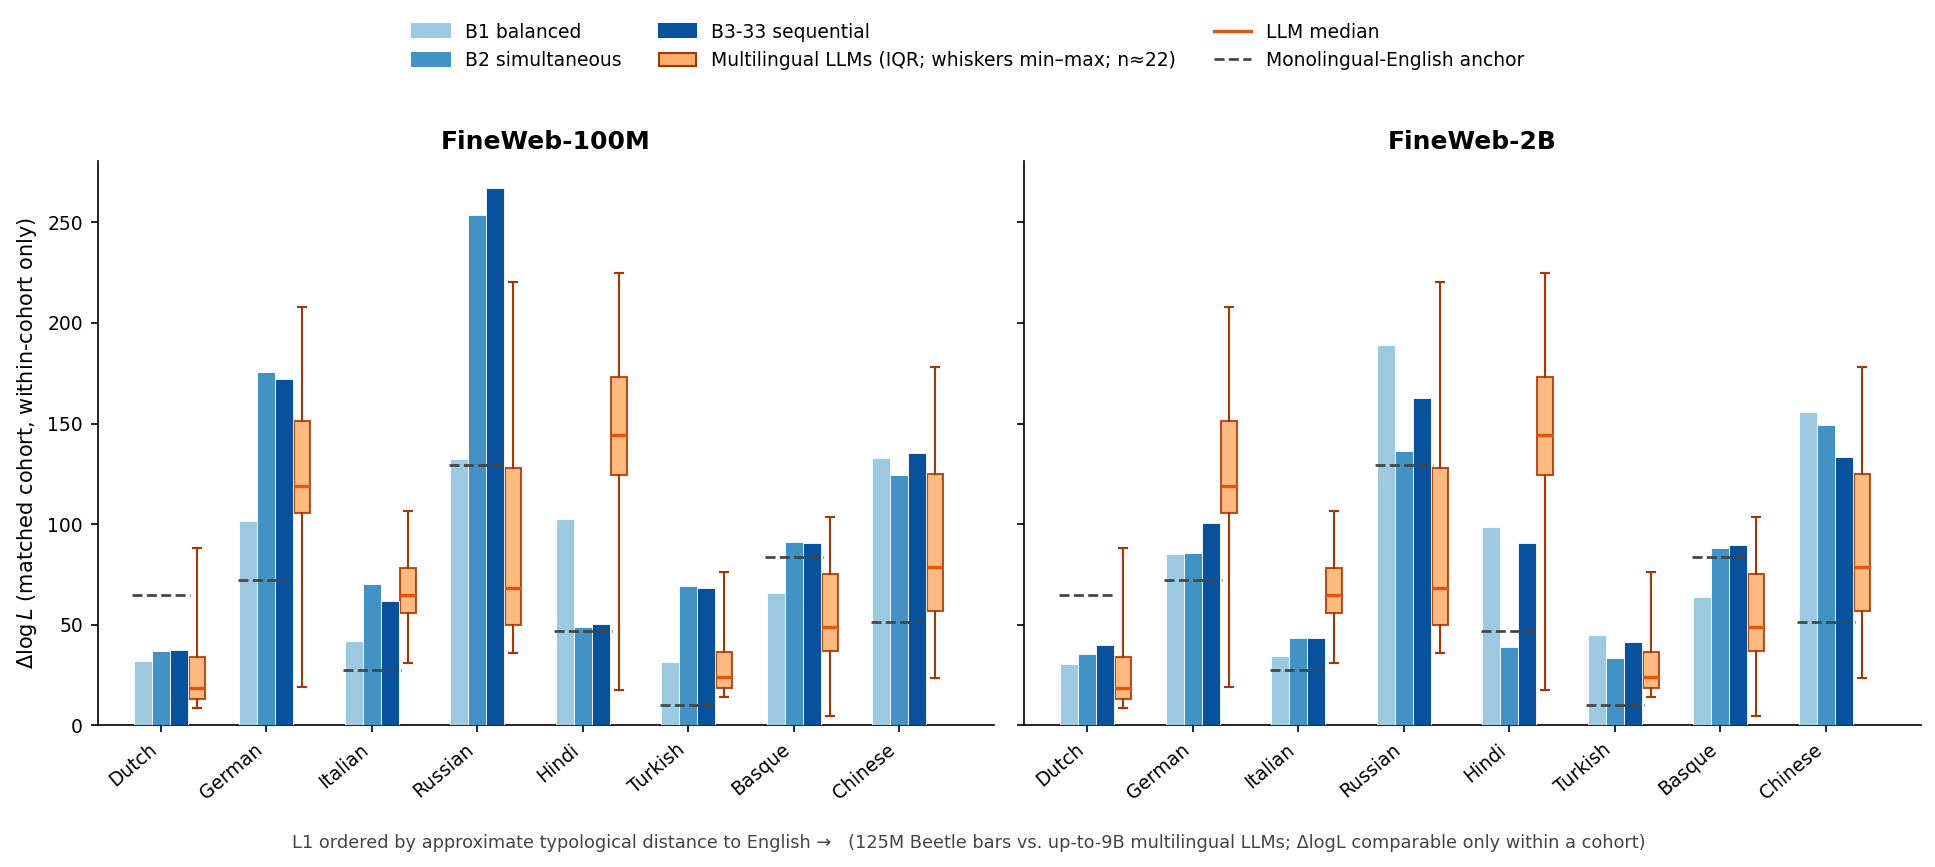
\includegraphics[width=\linewidth]{fig/meco/F4_per_l1_matched.png}
%     \caption{\textbf{Per-L1 matched L2 reading-time alignment vs.\ multilingual LLMs.} Across eight MECO L2 cohorts, small bilingual \beetle{} models (125M; B1–B3-33) achieve $\Delta\log L$ comparable to or exceeding a 22-model (150M–13B) multilingual LLM distribution, often outperforming the LLM median and matching or surpassing a monolingual-English anchor, with stronger gains at lower pretraining scale and reduced curriculum effects at higher scale.
%     }
%     \label{fig:meco-typ-l1-staged-balanced}
% \end{figure}


% Across all three MECO L1 reader cohorts, staged exposure curricula (B2, B3-33, B5) consistently outperform balanced bilingual exposure (B1) in explaining L2 reading-time variance, as reflected in per-L1 comparisons in App.~E. Two macro-level patterns frame these results. First, small bilingual models are already competitive with substantially larger multilingual LLMs: in most L1 cohorts, the 125M-parameter models fall within the upper range of the multilingual distribution and are often comparable to or better than the monolingual English anchor. Second, the advantage of staged over balanced exposure is scale-dependent, being more pronounced at smaller pretraining scale (FineWeb-100M) and weakening at larger scale (FineWeb-2B), suggesting that curriculum effects are strongest under data-limited conditions where learning dynamics are less saturated. Continual-learning overlays such as EWC and replay-based variants produced no robust improvement once the underlying exposure schedule was fixed (\autoref{fig:meco_two_col_layout}). 

% Three qualitative trends emerge consistently across cohorts. The benefits of staged curricula are concentrated in Germanic L1 readers (notably Dutch and German), consistent with typological proximity and stronger lexical overlap between training exposure and evaluation language structure. The improvements primarily affect early-stage reading-time measures associated with lexical access and initial integration, rather than later integrative processes such as regression-path duration (see \autoref{fig:meco_stage_dissociation}); this aligns with evidence that surprisal-driven effects are strongest in early eye-movement measures such as first-pass reading time and immediate spillover \citep{berzak2023eye, nahatame2025relative}. Finally, the effect attenuates for Chinese L1 readers, where ordering differences are weaker and less stable across scales, consistent with established typological distance effects in L2 reading. In particular, greater orthographic and structural mismatch reduces early predictive facilitation and shifts processing toward later integration stages \citep{kuperman2025distance, luke2023exgaussian, zhao2026proficiency}.

% We also test whether MECO performance depends on the proportion of L1:L2 and the ordering, changing the manner in which data is introduced in each '\beetle{}'s exposure schedules  (gradually introduced or in bursts). In Dutch, German and Chinese-English models, we find even when models see exactly the same amount L1 and L2 data, arranging it in structured phases (block staging) produces statistically significantly better MEOC alignment with human reading behaviour than interleaved, gradual, or shuffled exposure (\autoref{tab:tiso_main}, \autoref{fig:tiso_main_body}).  




%     %textbf{Per-L1 matched L2 reading-time alignment vs.\ the multilingual-LLM distribution.} Each L1's own bilingual \beetle{} model (B1 balanced, B2 simultaneous, B3-33 sequential; 125M params) evaluated on its own L1's MECO L2 readers, at two pretraining scales (FineWeb-100M, left; FineWeb-2B, right), for the eight L1s with both a trained model and a MECO reader cohort, ordered by approximate typological distance to English. Orange boxes summarise the per-cohort multilingual-LLM $\Delta\log L$ spread (IQR box, min--max whiskers, median line; $n{=}22$ LLMs, 150M--13B params); the dashed line is the monolingual-English \beetle{} anchor. LLM and monolingual baselines are scale-independent and hence identical across panels. At 125M params \beetle{} sits above the LLM median in 7/8 cohorts (exceeding all 22 LLMs on Russian), Hindi excepted, and above the monolingual anchor in 7/8 cohorts (Dutch excepted)---i.e.\ a small bilingual model is \emph{comparable to} much larger multilingual LLMs rather than uniformly better. Staged curricula (B2/B3-33) exceed balanced exposure (B1) in 7/8 cohorts at FineWeb-100M but only 4/8 at FineWeb-2B, indicating the curriculum effect concentrates at smaller scale. $\Delta\log L$ is comparable only within a cohort (same readers), so cross-cohort bar heights reflect cohort size, not effect size; full per-cell values in Tab.~\ref{tab:meco_per_l1_matched}.


% %Across Dutch, German, and Chinese L1 readers, staged schedules (B2, B3-33, B5) consistently outperform balanced exposure (B1) in explaining reading-time variance (Tab.~\ref{tab:meco_curriculum_matched} \textcolor{red}{missing reference}, Fig.~\ref{fig:meco-typ-l1-staged-balanced}). The effect is strongest for Dutch and German readers, where improvements concentrate in early measures associated with lexical access and immediate integration, including first-pass duration and spillover (Fig.~\ref{fig:fig3_spillover_decay}). For Chinese reader data, the ordering is weaker and less consistent, indicating reduced sensitivity to curriculum structure (Fig.~\ref{fig:fig9b_curriculum_sweep_matched} \textcolor{red}{missing reference}). At human scale, B3 yields higher $\Delta\log L$ than B1 for Dutch (139.6 vs. 62.3) and German (177.5 vs. 75.1), with B2 and B5 showing intermediate values (Tab.~\ref{tab:meco_curriculum_matched}). 
% %\textcolor{red}{Don't report the individual LLs. instead, guide the reader through the results and help them understand the conclusions.}


% %These differences are primarily reflected in first-pass measures such as first-run duration, with smaller separation in later-stage measures including regressions and refixations (Fig.~\ref{fig:fig3_spillover_decay}, Tab.~\ref{tab:sig_decomp_dissociation}). Spillover patterns show that staged curricula concentrate effects at lag 0, whereas B1 distributes effects across later lags (Fig.~\ref{fig:fig3_spillover_decay}). Detailed L1 results across curricula are in \autoref{fig:meco-typ-all-l1}. 


% %\textcolor{red}{if we're going to compare the different reading time metrics/analyses, we probably need to explain more about what the difference is between them a little bit more? (i defer to james on this)}

% %\begin{figure}[!ht]
%  %   \centering
%   %  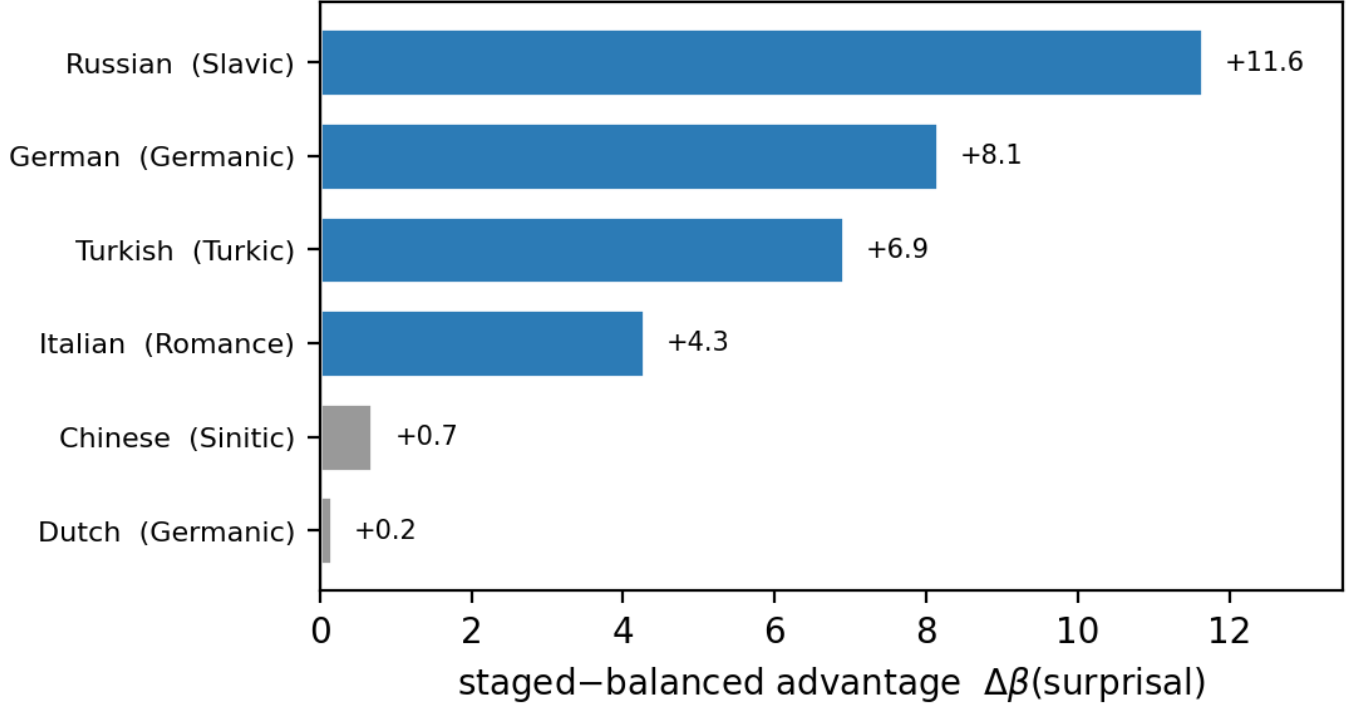
\includegraphics[width=1\linewidth]{fig/meco/meco-typ.png}
%    % \caption{\textbf{Staged v Balanced MECO Advantage by L1 Language Family}: Comparison of \beetle{} MECO Alignment for \texttt{balanced (B1)}  v \texttt{staged (B2 - B5)} curricula ($\Delta \mathrm{log}\,L$) across all \beetle{} models, grouped by L1 language family \textcolor{red}{[catherine: i think this staged/balanced advantage thing is a bit unintuitive to me. i think it's more interesting to explore either a) the relationship between this difference and the English proficiency of the MECO participants or b) the difference in the NLL scores between the languages (are the models better at predicting reading time when the performance between the 2 languages is more unbalaned?)]}}
%   %  \label{fig:meco-typ-l1-staged-balanced}
% %\end{figure}


% %\begin{figure}[!ht]
%  %   \centering
%   %  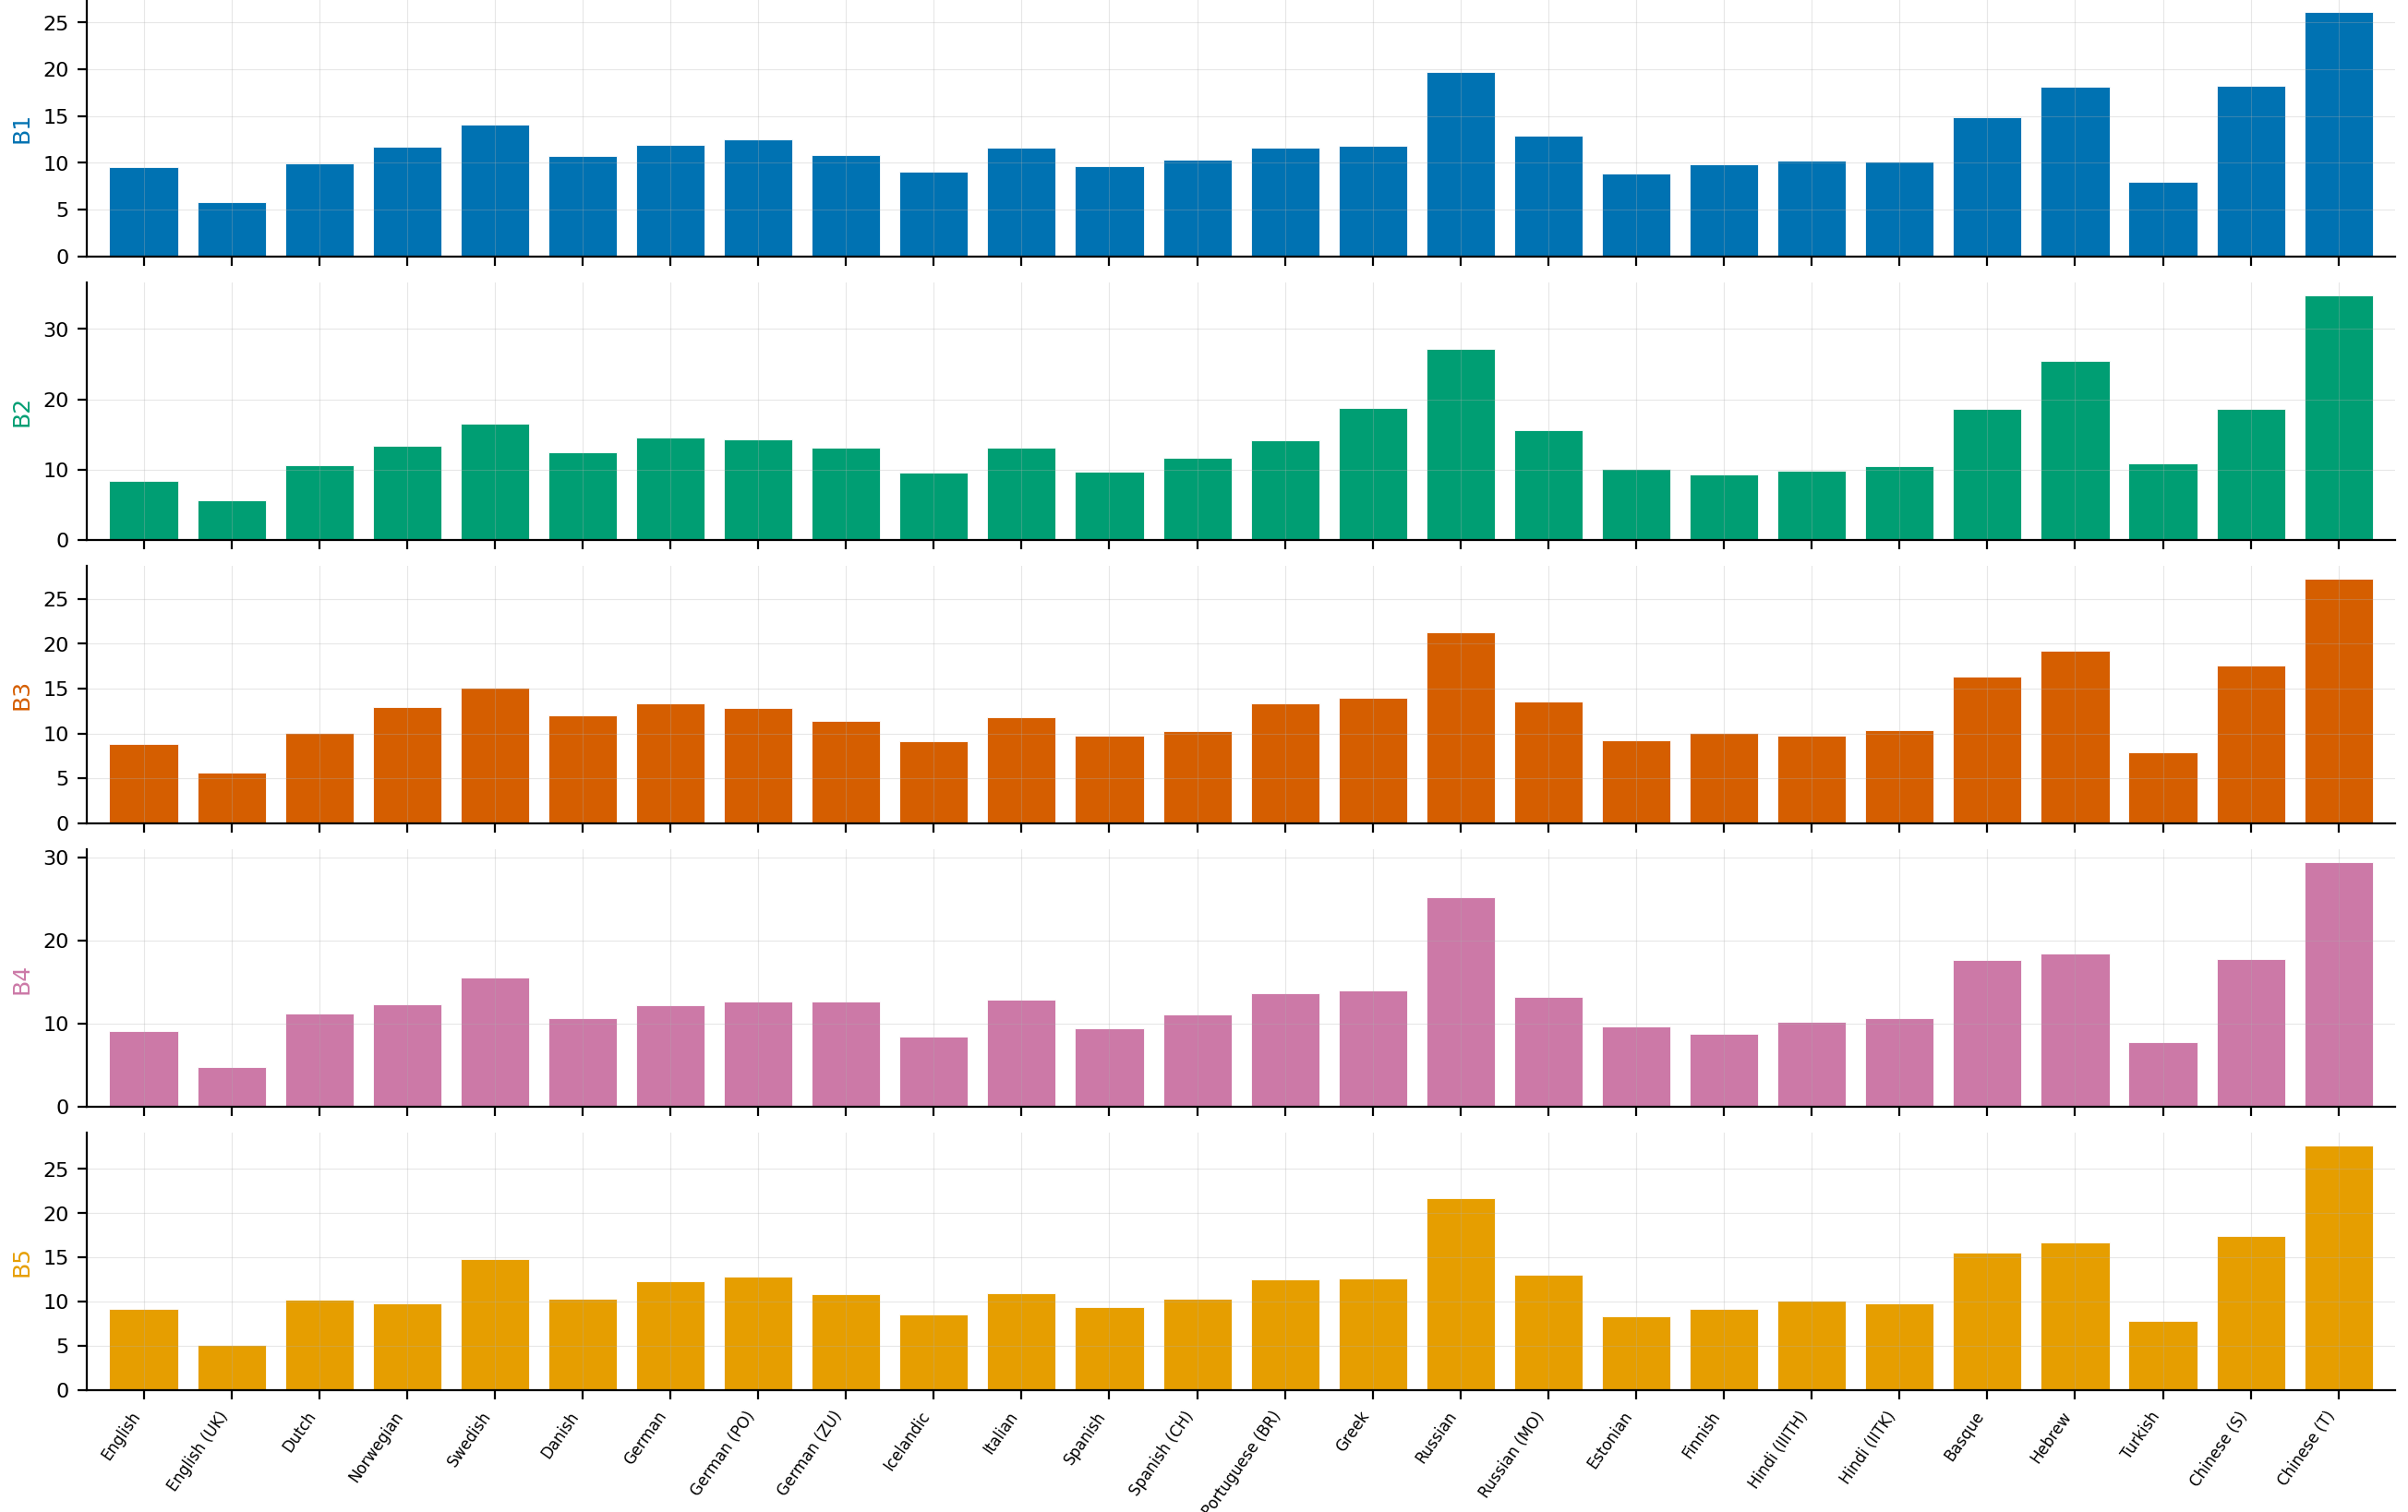
\includegraphics[width=1\linewidth]{fig/meco/meco_typ_curricula.png}
%    % \caption{\beetle{} 100M FineWeb MECO Alignment B1 - B5 ($\Delta \mathrm{log}\,L$) for L1 Dutch, Norwegian, Swedish, Danish, German, Icelandic, Spanish, Portuguese, Greek, Russian, Estonian, Hindi, Basque, Hebrew, Turkish Chinese \textcolor{red}{[catherine: again, because there are no baselines here, I don't think it makes sense to report these in the main text. it might be better to make a figure with just the B2 or B3 curriculum results and then compare against the best multilingual model (and maybe the monolingual baseline model), so we can see how often our models beat the baselines.]}}
%     %\label{fig:meco-typ-all-l1}
% %\end{figure}


% %Across Dutch, German, and Chinese L1 readers, staged schedules (B2, B3-33, B5) systematically outperform balanced exposure (B1) in explaining reading-time variance. The improvement is largest for Dutch and German readers, concentrating in early measures tied to lexical access and immediate integration (first-pass duration and spillover). For Chinese readers the ordering is weaker and less consistent, indicating reduced sensitivity to curriculum structure.


% %The primary result comes from the matched-diagonal curriculum comparison (Tab.~\ref{tab:meco_curriculum_matched}, with full breakdowns in App.~\ref{sec:meco-results}, Tabs.~\ref{tab:meco_langrows}--\ref{tab:meco_full_canonical}), which holds architecture, tokenizer, data, and reader cohort fixed and varies only exposure schedule. Across Dutch, German, and Chinese L1 readers, staged curricula (B2 simultaneous, B3-33 sequential, B5 late-onset) consistently outperform balanced exposure (B1) in aligning surprisal with human first-pass reading times. At human scale, B3-33 reaches $\Delta\log L = 139.6$ for Dutch readers versus $62.3$ for B1, and $177.5$ versus $75.1$ for German readers (Tab.~\ref{tab:meco_curriculum_matched}). Gains concentrate in early reading measures associated with lexical access and initial integration. Relative to B1, staged curricula increase first-run sensitivity ($+0.79$~SD, $95\%$ CI $[+0.24, +1.33]$ for B2; $+0.93$~SD $[+0.43, +1.42]$ for B5) while reducing late-stage effects such as regressions and refixations (App.~\ref{sec:meco-stage-app}, Tab.~\ref{tab:sig_decomp_dissociation}). This shift is mirrored in spillover structure: staged curricula concentrate surprisal effects at lag~0, whereas B1 distributes effects across later lags (Fig.~\ref{fig:fig3_spillover_decay}). The ordering is robust against a monolingual-English anchor under the matched specification in App.~\ref{sec:meco-stage-app}, where B3-33 approaches monolingual performance for Dutch ($\approx 139$), B2 is comparable ($\approx 136$), and B1 lags substantially. Effects attenuate with typological distance from English, being strongest for Germanic readers and weaker for Chinese (Fig.~\ref{fig:fig9b_curriculum_sweep_matched}).


% %Across Dutch, German, and Chinese L1 readers, we observe a consistent curriculum effect: \textbf{staged exposure schedules (B2, B3-33, B5) systematically outperform balanced exposure (B1)} in explaining reading-time variance. This improvement is most pronounced for Dutch and German readers, where gains concentrate in early reading measures associated with lexical access and immediate integration (first-pass duration and spillover). For Chinese readers, the same ordering is weaker and less consistent, indicating reduced sensitivity of alignment to curriculum structure in this setting. Importantly, these differences persist across training scales (100M–24B tokens), suggesting that the effect is not driven by data quantity but by the \textbf{structure of exposure over time}. MECO results indicate that structured bilingual curricula shift models toward better prediction of early-stage reading behaviour, consistent with an emphasis on short-horizon lexical expectations in surprisal.


% %Across Dutch, German, and Chinese L1 readers, we observe a consistent curriculum effect: \textbf{staged exposure schedules (B2, B3-33, B5) outperform balanced exposure (B1}) in explaining reading-time variance. The effect is strongest for Dutch and German, which are more typologically similar to English, where gains are concentrated in early processing measures (first-pass duration and immediate spillover).  The fit is weaker for more distant Chinese, which is more distant from English.. Importantly, curriculum differences persist across training scales (100M--24B tokens), indicating that the effect is not reducible to data size but to exposure structure. MECO results suggest that structured bilingual exposure primarily modulates early lexical-access dynamics in L2 reading, consistent with a shift toward shorter-horizon predictive information in surprisal. Fig.~\ref{fig:meco_curriculum} shows the curriculum sweep across Dutch, German, and Chinese reader populations. On the matched Dutch-reader condition, B3 Dutch-English Human-Scale reaches $\Delta\log L=\mathbf{139.6}$, compared with 62.3 for balanced B1. On the matched German-reader condition, B3-33 deu--eng HS reaches $\mathbf{177.5}$, while B1 achieves only 75.1. Chinese shows a weaker curriculum effect overall, with B5 zho--eng HS reaching the strongest matched result ($115.4$). Full matched-L1 curriculum results are reported in Tab.~\ref{tab:meco_curriculum_matched}. The curriculum effect attenuates monotonically with typological distance from English (App.~Fig.~\ref{fig:bA8_typology_per_curriculum}). Dutch and German readers exhibit the largest separation between staged and balanced curricula, while the Chinese-reader condition is substantially compressed. This typological gradient is consistent across both HumanScale and FineWeb training scales.


% %\textbf{Exposure \emph{order}, not mixture, drives the reading-time gain.} Five exposure schedules share an identical $50\%$-English token mixture and differ only in \emph{staging}---how English is arranged in time (\emph{top:} realised English share over training, colour-coded per arm), from no staging (T0 constant) to maximal staging (T3 block, English in the second half). \emph{Bottom:} MECO reading-time fit $\Delta\log L$ for every arm and training pair, each model scored against its matching L1 reader cohort; the staged arm (T3 block) is best in all three cohorts. Bars are seed means (whiskers $95\%$ CI, dots per seed) where replicated---nld--eng $n{=}5$ for all arms, deu/zho T0 and T3 $n{=}3$; the deu/zho T1/T2/T4 cells are single-seed reduced-config runs (bars only). $\Delta\log L$ is comparable only \emph{within} a cohort. Significance and exact magnitudes: Tab.~\ref{tab:tiso_results}.
% \begin{figure}[!t]
%   \centering
%   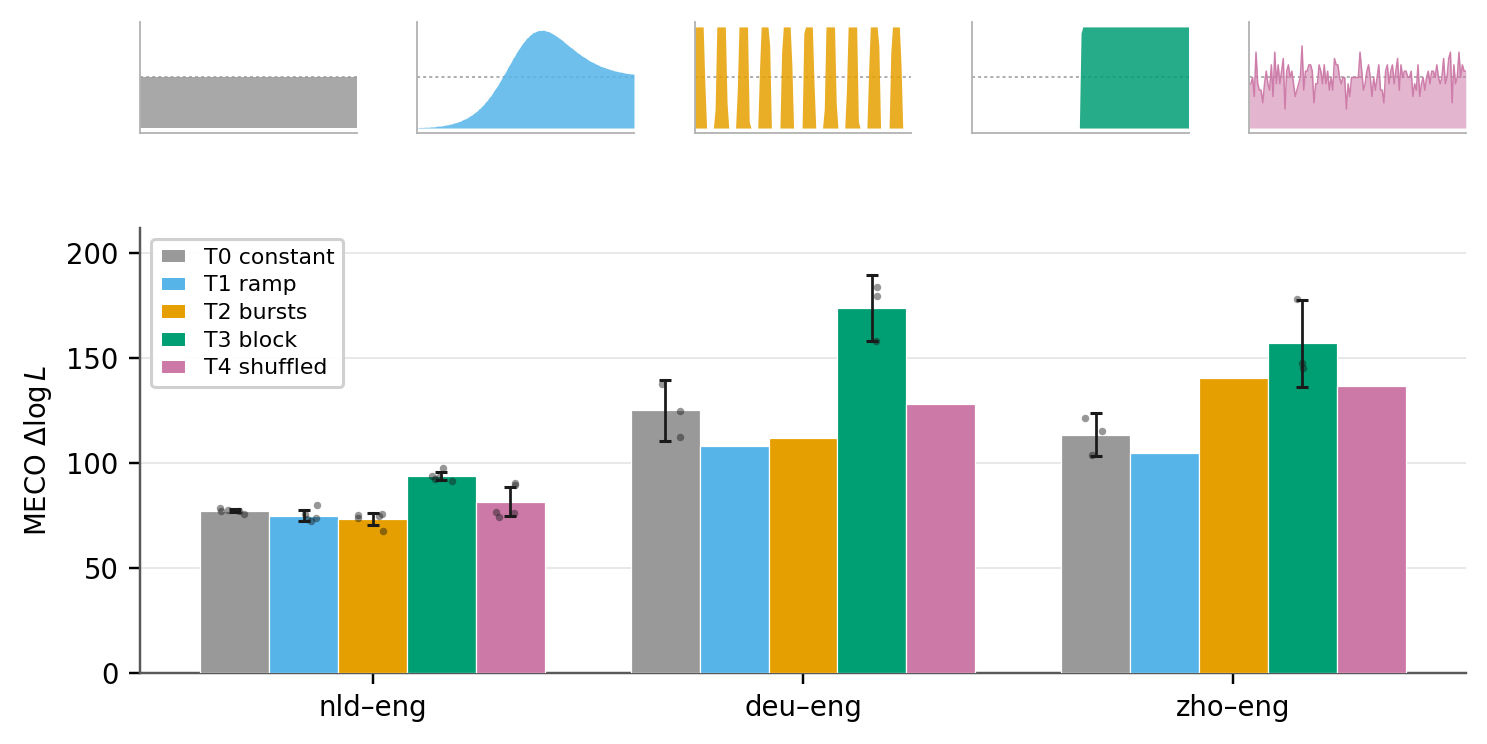
\includegraphics[width=\linewidth]{fig/meco/tiso_meco_final_appendix.png}
%   \caption{\textbf{Exposure \emph{order}, not mixture, drives the reading-time gain.} \textcolor{red}{1) figure descriptions should help you interpret the figure, not provide discussion/conclusions about the results 2) i disagree with this interpretation. it's about the mixture here, since the overall proportion is the same across both and the one with the sequential mixture is the most predictive}}
%   \label{fig:tiso_main_body}
% \end{figure}

% \begin{table}[!ht]\centering\small
% \caption{\textbf{Timing isolation ($n{=}5$).} nld--eng HumanScale, MECO Dutch readers, mean$\pm$sd over five training seeds at a fixed token marginal ($0.50$); only temporal order differs. The structure contrast (T3$-$T0${=}16.6$) and the order contrast (T3$-$T4${=}12.4$) are both significant at the seed level ($p{<}.001$ and Holm $p{=}.008$) and the reader level ($p{<}10^{-4}$). Full per-cohort results in App.~Tab.~\ref{tab:tiso_results}.}
% \label{tab:tiso_main}
% \begin{tabular}{llc}
% \toprule
% Arm & Schedule & $\Delta\log L$ \\
% \midrule
% T0 & constant (IID) & $77.1\pm0.9$ \\
% T3 & block staging & $\mathbf{93.7\pm2.4}$ \\
% T4 & shuffled order & $81.3\pm7.9$ \\
% \bottomrule
% \end{tabular}
% \end{table}


% \begin{figure}[t]
%   \centering
%   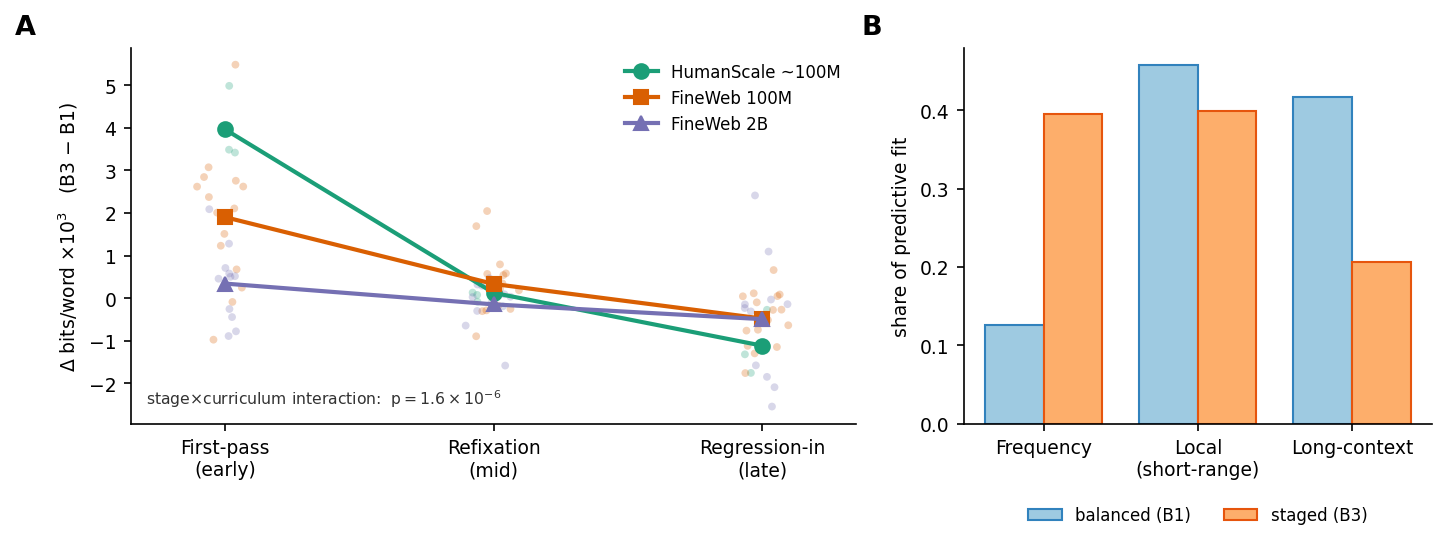
\includegraphics[width=0.85\linewidth]{fig/meco/processing_stage_dissociation.png}
%   \caption{\textbf{Exposure structure redistributes predictive information across reading-processing stages rather than improving alignment uniformly.} \textbf{(A)}~Stage-resolved staged$-$balanced $\Delta\log L$ change, showing the early$\to$late sign reversal. \textbf{(B)}~The convergent context-share decomposition (as Fig.~\ref{fig:D5_decomp_shares}, Tab.~\ref{tab:sig_decomp_curriculum}). Full statistics in App.~\ref{sec:reading-time-stage}.}
%   \label{fig:meco_stage_dissociation}
% \end{figure}

% \subsection{Curriculum effects persist across scale}

%  \autoref{fig:meco_two_col_layout} shows that curriculum effects are stable across budgets (100M--24B): staged schedules, especially B3-33 and B5, maintain a stronger surprisal--reading-time coupling than B1 , though the effect is not uniform across languages and scales. Dutch shows consistent gains at all model sizes, German exhibits a single exception at 2B (B5), and Chinese does not show a stable dominance pattern. \autoref{fig:meco-typ-l1-staged-balanced} compares the MECO alignment 100M and 2B B1 - B3 for 8 L1s, suggesting that curriculum effects are  strongest at human scale,  but weakens at 2B. 

% %The curriculum ordering is stable across training budgets, with staged schedules---in particular B3-33 and B5---consistently achieving stronger surprisal–reading-time coupling than balanced exposure from human-scale (100M) through FineWeb-scale (24B) training (Fig.~\ref{fig:fig_meco_best_of_family}). This advantage is not uniform across languages or scales. Dutch shows a stable benefit for staged curricula across all scales, German shows one exception (B5, 2B tokens), and Chinese shows no consistent curriculum dominance (Tab.~\ref{tab:meco_curriculum_matched}). Across scales, the effect is therefore sign-consistent but magnitude-dependent: staged curricula perform strongly at human scale, weaken at 2B (where gains for Germanic L1s are offset by reversals in Chinese), and partially recover at 24B, remaining positive in aggregate (Tab.~\ref{tab:hier-contrasts}, Fig.~\ref{fig:hier-forest}). This pattern is consistent across L1 language families on the surprisal axis (Fig.~\ref{fig:l1_generality}). We quantify this advantage as a data-efficiency effect: staged curricula reach MECO alignment comparable to BLOOM-7.1B at substantially lower training tokens. \textcolor{red}{[catherine: i think this is kind of a weird comparison to make because of the phase transition/2B token thing. based on other work, we would expect larger models to model reading time worse, so reaching the level of a 7B model might not necessarily be the best comparison.]} This resembles the training-dynamics transition reported for monolingual psychometric alignment by \citet{aoyama-wilcox-2025-language}, but emerges earlier under structured bilingual exposure. Continual-learning overlays such as EWC and replay-based variants produced no robust improvement once the underlying exposure schedule was fixed (App.~\ref{sec:sig-robustness}), suggesting that the temporal organisation of bilingual exposure therefore appeared more influential than the particular continual-learning regulariser used to implement it.

% %\textbf{.} The curriculum ordering is stable across training budgets. Staged schedules — B3-33 and B5 in particular — maintain stronger surprisal–reading-time coupling than balanced exposure from human-scale (100M) through FineWeb-scale (24B) training, and the B3-33/B5 advantage compounds with additional training (Fig. 3a). We quantify this as an efficiency gain: staged curricula exceed the MECO alignment of BLOOM-7.1B at a small fraction of its training tokens. This resembles the training-dynamics transition reported for monolingual psychometric alignment by \citet{aoyama-wilcox-2025-language}, but emerges substantially earlier under structured bilingual exposure. 



% %The curriculum ordering remains stable across training-token budgets. Staged schedules (B3-33 and B5 in particular) maintain stronger surprisal–reading-time coupling than balanced exposure from small-scale (100M) through large-scale (24B) training. At a qualitative level, this suggests that structured exposure schedules produce an efficiency gain in learning reading-aligned predictive structure: improvements emerge early in training and persist rather than depending on continued scaling. The curriculum ordering remains stable across training-token budgets (App.~Fig.~\ref{fig:fig1_scaling_x_curriculum}). Sequential and late-onset curricula maintain stronger surprisal--reading-time coupling than balanced exposure from HumanScale~100M through FineWeb-scale training. Fig.~\ref{fig:meco_efficiency} shows that staged \beetle{} curricula exceed the MECO alignment achieved by BLOOM7.1B at a fraction of its training budget, and that the B3-33/B5 advantage compounds with additional training. This pattern resembles the training-dynamics transition reported for monolingual psychometric alignment by \citet{aoyama-wilcox-2025-language}, but emerging substantially earlier under structured bilingual exposure.


% \subsection{Comparison of \beetle{} and Multilingual LLMs}
% \label{sec:meco-vs-multilingual}

% 125M \beetle{} models achieve MECO reading-time alignment that is comparable to, and in several cohorts exceeds, multilingual LLMs ranging up to 13B parameters, with staged curricula reaching the BLOOM-7.1B regime at substantially lower training budgets (Tab.~\ref{tab:meco_baseline_comparators}, Fig.~\ref{fig:meco_efficiency}). Despite their small scale, these bilingual models consistently occupy the upper portion of the multilingual LLM distribution, exceeding the LLM median in 7/8 L1 cohorts and surpassing all evaluated LLMs in Russian, while remaining below the monolingual English anchor only in isolated cases. Across L1 groups, \beetle{} models trained with staged exposure (B2/B3-33) consistently outperform balanced exposure (B1), particularly at smaller pretraining scale (FineWeb-100M), indicating that curriculum structure can substitute for parameter scale in shaping alignment. This effect is not uniform across languages: gains are strongest for Dutch and German readers, while weaker or inconsistent effects are observed for Chinese readers, suggesting systematic L1-dependent sensitivity in how exposure order influences L2 reading-time alignment (Tab.~\ref{tab:meco_english_l2_participants}).

% %125M \beetle{} models achieve MECO alignment comparable to or exceeding multilingual LLMs up to 9B parameters, with staged curricula reaching the BLOOM-7.1B regime at substantially lower training budgets (Tab.~\ref{tab:meco_baseline_comparators}, Fig.~\ref{fig:meco_efficiency}). Across L1 groups, \beetle{} models consistently occupy a higher alignment regime than balanced exposure baselines, indicating that training structure, rather than parameter scale alone, drives alignment differences. The strongest gains are observed for Dutch and German readers, with weaker effects for Chinese readers, indicating systematic L1 dependence (Tab.~\ref{tab:meco_english_l2_participants}).

% %Comparing \beetle{} to multilingual LLMs, \beetle{} achieves comparable or stronger alignment at far smaller budgets: the LLMs vary little across architectures and scales and sit in a lower alignment regime, while Beetle occupies a consistently higher regime across all L1 groups and curricula. MECO alignment is therefore not explained by parameter scale alone but by training structure. The L1 dependence is consistent throughout — gains strongest for Dutch and German, weakest for Chinese — indicating that the benefit of structured exposure interacts with typological proximity to English rather than improving alignment uniformly.


% %Comparing \beetle models  and multilingual LLMs,  \beetle models achieve comparable or stronger alignment at substantially smaller training budgets. Multilingual LLM pretrained model performance on MECO is comparatively lower than \beetle{} models. Multilingual LLMs show relatively small variation across architectures and scales. In contrast, \beetle{} models consistently occupy a higher alignment regime across all L1 groups and curricula.  This suggests MECO alignment is not explained by parameter scale alone, but by training structure: models trained with staged bilingual exposure exhibit stronger coupling between surprisal and human reading times.  A second consistent pattern is \textbf{L1 dependence}. Gains are strongest for Dutch and German readers, while Chinese readers show weaker separation between curricula and baselines. This indicates that the benefit of structured bilingual exposure interacts with typological proximity to English rather than reflecting a uniform improvement across languages.





% %\textcolor{red}{This section feels more complicated than it needs to be. Can you streamline it so it gets only the main points across?}
% %The \beetle{} models consistently outperform much larger multilingual LLMs on aggregate MECO reading-time alignment. The multilingual-LLM aggregate means are 19.57 / 119.01 / 80.69 (n=10 models; Tab.~\ref{tab:meco_full_canonical}), substantially lower than the corresponding \beetle{} averages (mean over 33 curriculum and scale variants) of 81.10 / 167.04 / 130.41. This gap is robust across curriculum variants and is not explained by scale alone: even the strongest multilingual baseline remains well below the smallest structured bilingual models on these aggregate MECO alignment measures. In particular, \beetle{} variants such as B3-33 (nld--eng) exceed BLOOM-7b1 by approximately 7.1× on Dutch MECO $\Delta \log L$ (139.58 / 19.69 = 7.09), consistent with the appendix-level analyses. Rather than indicating a simple scaling effect, structured bilingual exposure is associated with a shift in predictive mass toward shorter-horizon lexical expectations that more closely resemble human early reading behaviour. This pattern is strongest for Dutch and German L1 readers and is substantially reduced for the Chinese reader group, consistent with an interaction between L1 similarity and curriculum-induced predictability structure (cf. Appendix~\ref{sec:bA8}). Overall, these results suggest that bilingual exposure structure is more predictive than model scale alone for alignment with human reading dynamics in this setting.

% \subsection{Why does exposure scheduling affect L2 reading time prediction?}

% %\textbf{.} Curriculum effects concentrate on early reading measures associated with lexical access rather than later integrative processes, suggesting that exposure structure reshapes how models distribute predictive information across time scales. One interpretation is that staged curricula encourage greater reliance on short-horizon lexical and local-context predictions, which align more closely with first-pass reading, whereas balanced exposure retains more long-context dependency that contributes less to early reading-time variance. This is consistent with the observed pattern — gains in early measures, attenuation in later spillover-sensitive components — pointing to a shift in the locus of predictive information rather than a uniform improvement across processing stages. Full results, mixed-effects models, significance tests, spillover analyses, and participant-level breakdowns appear in  App.~\ref{sec:meco-results} and App.~\ref{sec:significance-comprehensive}.

% %Curriculum effects are strongest on early reading measures associated with lexical access rather than later integrative processes. This suggests that exposure structure primarily reshapes how models distribute predictive information across time scales. One way to interpret this is that staged curricula encourage models to rely more heavily on \textbf{short-horizon lexical and local-context predictions}, which are more closely aligned with the dynamics of first-pass reading. In contrast, balanced exposure retains relatively more long-context dependency in its predictive structure, which contributes less directly to early reading-time variance. This interpretation is consistent with the observed MECO pattern: gains are concentrated in early measures and are attenuated in later spillover-sensitive components, indicating a shift in the locus of predictive information rather than a uniform improvement across processing stages. We provide detailed MECO results, mixed effect models,  significance tests, spillover analyses, and participant-level breakdowns in App.~\ref{sec:meco-results} and App.~\ref{sec:significance-comprehensive}.


%  %Relative to balanced exposure (B1), staged curricula improve prediction of first-run duration while reducing alignment with later measures such as refixations and regressions-in (App.~\ref{sec:meco-stage-app}). Fig.~\ref{fig:fig3_spillover_decay} shows that staged curricula concentrate surprisal effects at lag~0, whereas balanced exposure produces a flatter spillover profile distributed across later lags. 

% %Reading-time alignment reflects a mixture of lexical access, local syntactic prediction, and contextual integration \citep[][add citations]{}, so a curriculum effect on MECO~L2 alignment could in principle arise from any of these processing levels. This suggests that structured bilingual exposure redistributes predictive mass toward shorter-horizon lexical expectations that more closely resemble human early reading behaviour. 

% Across MECO L2 reading-time evaluations, staged exposure curricula consistently outperform balanced bilingual exposure in aligning model predictions with early-stage human reading behaviour. At the primary level of analysis (first-pass reading time), staged curricula yield a robust improvement in model fit (e.g., $\Delta \log L = +3.96$ at HumanScale and $+1.90$ at FineWeb-100M in $\Delta$ bits/word $\times 10^3$), with the staged-versus-balanced contrast reaching statistical significance under a cluster-robust Wald test ($p = 1.6 \times 10^{-6}$) and corroborated by a nonparametric Friedman test across cohorts ($p = 3.6 \times 10^{-3}$). This effect is consistent across reader populations (26/30 cohorts show a positive direction), but is modulated by scale, attenuating and becoming non-significant at larger model sizes ($p = 0.24$ at 2B scale), indicating a size-dependent interaction.  A stage-resolved analysis further reveals a significant stage $\times$ curriculum crossover (early vs.\ late measures: $p = 2.7 \times 10^{-7}$), whereby staged exposure improves alignment for early first-pass measures while reducing fit to later integration signals such as regressions-in probability. This pattern is supported by a redistribution in predictive contributions, with the long-context share of predictive power decreasing from 0.43 under balanced exposure to 0.18 under staged curricula (permutation $p < 10^{-4}$), accompanied by a compensatory increase in unigram- and frequency-driven contributions. Together, these results indicate a statistically reliable shift in predictive strategy induced by exposure scheduling, rather than a uniform improvement in reading-time alignment.

% %\textcolor{red}{\textit{shorter version}Reading-time alignment reflects a mixture of lexical access, local syntactic prediction, and contextual integration \citep{hopp2016timing,hofmann2022language,shain2024large}, so a curriculum effect on MECO~L2 alignment could in principle arise from any of these processing levels. This suggests that structured bilingual exposure redistributes predictive mass toward shorter-horizon lexical expectations that more closely resemble human early reading behaviour. Relative to balanced exposure (B1), we find staged curricula improve prediction of first-run duration while reducing alignment with later measures such as refixations and regressions-in (App.~\ref{sec:meco-stage-app}). Fig.~\ref{fig:fig3_spillover_decay} shows that staged curricula concentrate surprisal effects at lag~0, whereas balanced exposure produces a flatter spillover profile extending into later lags. Together, these results indicate that exposure structure shifts predictive computation away from longer-horizon contextual integration and toward early lexical-access signals that dominate first-pass reading.}


% \clearpage



%tab:beetle_main,


%\textcolor{red}{I think we should add back in the multiblimp evals.}


% \begin{table}[t!]
% \centering
% \small
% \begin{tabular}{@{}llllll@{}}
% \toprule
%  & \multicolumn{5}{c}{\textbf{L1}}      \\ \midrule
%    & \texttt{nld} & \texttt{deu} & \texttt{ita} & \texttt{rus} & \texttt{eus} \\ \cmidrule(l){2-6}
% \textbf{B1} & 63.9 & 63.6 & 62.7 & 60.9 & 62.1 \\
% \textbf{B2} & 57.6 & 52.8 & 53.7 & 53.7 & 52.6 \\
% \textbf{B3} & 57.4 & 54.8 & 54.3 & 53.4 & 54.0 \\
% \textbf{B4} & 58.4 & 57.1 & 56.1 & 55.9 & 56.0 \\
% \textbf{B5} & 62.8 & 62.7 & 61.6 & 60.0 & 60.7 \\ \bottomrule
% \end{tabular}
% \caption{\beetle{} English BLiMP Accuracy for 100M FineWeb models across 5 L1s and 5 exposure curricula. Full Monolingual and Multi-BLiMP accuracies for the \beetle{} models are in \textit{Appendix} }
% \end{table}




%Measured as the change in FLORES-200 L1 perplexity against a matched monolingual anchor (Tab.~\ref{tab:forgetting}), the shifts reflect curriculum-modulated \emph{transfer}, not catastrophic forgetting \citep{kirkpatrick2017overcoming}. They separate two effects that raw L1 perplexity conflates: \emph{positive transfer}, where shared structure lets English exposure \emph{lower} L1 perplexity (Dutch shows sign reversals, $+2\%$ to $-20\%$; \citealp{whitford2015second}), and \emph{interference}, where capacity competition \emph{raises} it (German rises smoothly with staging strength, $+15\%$ to $+84\%$; Chinese, the most distant L1, degrades uniformly with no reversal)

%The interference is therefore graded and typologically gated---partly offset by transfer for Germanic L1s, uniform and unrecovered for Chinese---rather than catastrophic forgetting, which is confined to the diverging cells in App.~\ref{sec:downstream}.}


%In this section, we demonstrate that our training method induces  curriculum-dependent changes in model behaviour. 

%paragraph{Curriculum effects on per-token NLL.} In order to evaluate how model performance changes for both languages over the course of training, we measure next-token prediction at each checkpoint. Following \citet{chang2024goldfish}, we calculate the mean sentence-level NLL for FLORES items. This allows us to compare across models and across languages. \textcolor{red}{check this}
% We first examine whether per-token NLL evolves consistently with the structure of each exposure curriculum. Because all models share identical architecture, data, and training budgets, differences in FLORES-200 surprisal primarily reflect differences in when and how L1/L2 exposure is introduced rather than differences in overall optimisation dynamics. 
%\autoref{fig:flores_curves} shows that the models trained with different curricula show expected effects: early-exposure curricula diverge earlier from monolingual-like trajectories and delayed-onset curricula initially track similar curves before separating later. 

%\paragraph{Cross-lingual interference.} We also assess whether bilingual training degrades L1 modelling quality. We measure L1 retention as the change in FLORES-200 L1 perplexity \textcolor{red}{NLL?} relative to a matched monolingual anchor (Tab.~\ref{tab:flores_bi} \textcolor{red}{[missing reference]}; per-schedule summary in Tab.~\ref{tab:forgetting}). For German, the increase in L1 perplexity rises smoothly with interference strength (from $+15\%$ in balanced exposure, CF log-ratio $+0.14$, to $+40\%$ under sequential onset and $+84\%$ under simultaneous onset), whereas Dutch follows the same ordering but at smaller or inverted magnitude (approximately $+2\%$ in balanced exposure and $-20\%$ under sequential/late-onset settings), with both model families showing systematic cross-lingual transfer effects, rather than catastrophic forgetting. \textcolor{red}{[catherine: what about Chinese? what does this actually tell us about interference? seems like you can maybe make a case for positive transfer, but not necessarily interference?]}


%\textcolor{red}{this section is really confusing. i think it needs to be split more clearly into the different evals/tasks. we need to tell the reader what the evals are telling us/motivate why we're looking at things. and what's the main goal/takeaway for the results we're reporting? i think one of them should just be to demonstrate that overall the models are reasonable. i think it's good to make predictions about what the NLL curves should look like for each curriculum and show that they kind of look like that. most other things are not relevant to this paper.}

%To evaluate the quality of our models, we report loss curves over training and minimal pair linguistic knowledge benchmarks performance. We use MultiBLiMP \citep{jumelet2025multiblimp} for Dutch, German, French, Persian, and Bulgarian; BLiMP-NL \citep{suijkerbuijk-etal-2025-blimp-nl} for Dutch; and ZhoBLiMP \citep{liu-etal-2025-zhoblimp} for Chinese. 

%B3 Dutch--English FineWeb models reaches $90.3\%$ on Dutch MultiBLiMP (Table~\ref{tab:multiblimp}, App.~\ref{sec:downstream}) and surpasses the matched monolingual Dutch Beetle baseline at roughly 200M tokens.  We observe \ a $\Vert W_{OV}\Vert_F$ sign flip between English BLiMP ($r{=}{+}0.52$) and Dutch BLiMP ($r{=}{-}0.67$) along the B1$\leftrightarrow$B5 axis.  \emph{Convergence.} Fig.~\ref{fig:flores_curves} plots mean FLORES-200 per-token surprisal (nats/tok, equivalently log-perplexity) by curriculum, showing trajectories that separate by schedule shape rather than token budget alone, consistent with the B-GPT findings in Fig.~2 of \citet{arnett-etal-2025-acquisition}. \emph{Forgetting.} The per-curriculum catastrophic-forgetting results are reported in App.~\ref{sec:downstream} (Tab.~\ref{tab:forgetting}). On the German models, the B1 balanced curriculum incurs the smallest L1 perplexity penalty relative to the matched monolingual anchor (CF log-ratio $+0.14$ versus $+0.34$ to $+3.14$ for the remaining schedules). The largest penalty occurs under the B5 late-onset schedule, with mean $\Delta$-PPL against the German monolingual model reaches approximately ${\sim}118{,}800$ across $N{=}4$ models --- around ${\sim}750{\times}$ the B1 cost of 157 --- making it the only German configuration in Tab.~\ref{tab:forgetting} to exhibit absolute L1 forgetting at levels routinely observed in the Dutch and Chinese cells. The FLORES trajectories (Fig.~\ref{fig:flores_beetle_vs_bgpt}) further show that no \beetle{} curriculum exceeds the Dutch FLORES BPB divergence observed in the B-GPT \textsc{nl-en} sequential condition (11.45 BPT). On the Dutch and Chinese models, however, the lowest-forgetting curriculum is language-dependent (Heritage for Dutch and Simultaneous for Chinese).



% \begin{figure}[t]
%     \centering
%     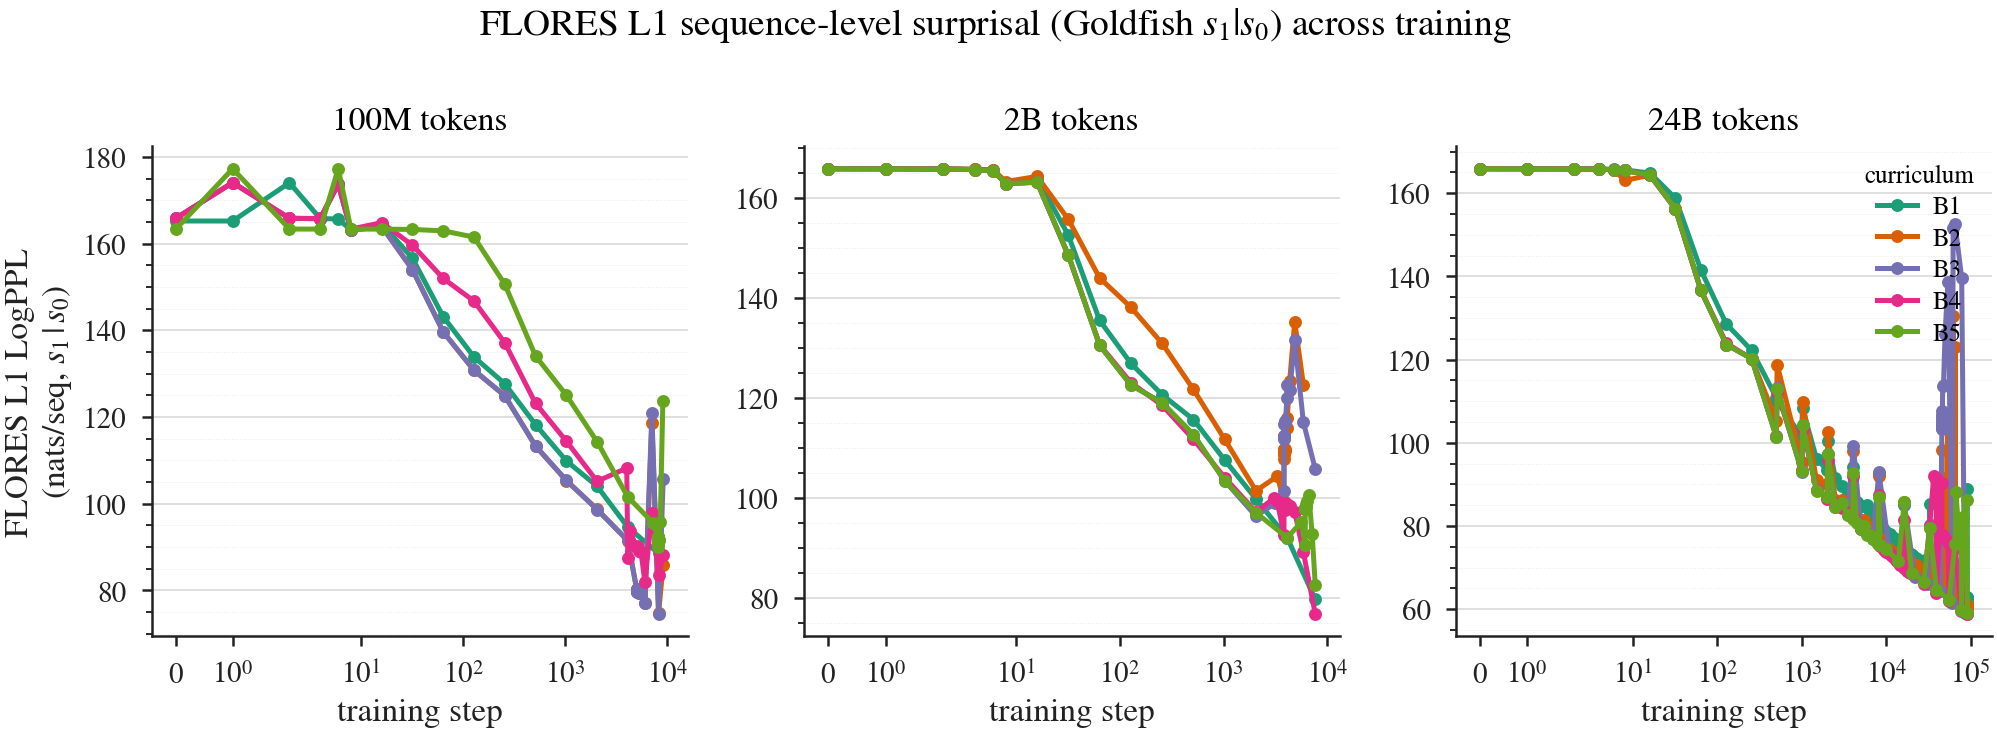
\includegraphics[width=\linewidth]{fig/flores/beetle-flores-l1_v2.png}\\
%     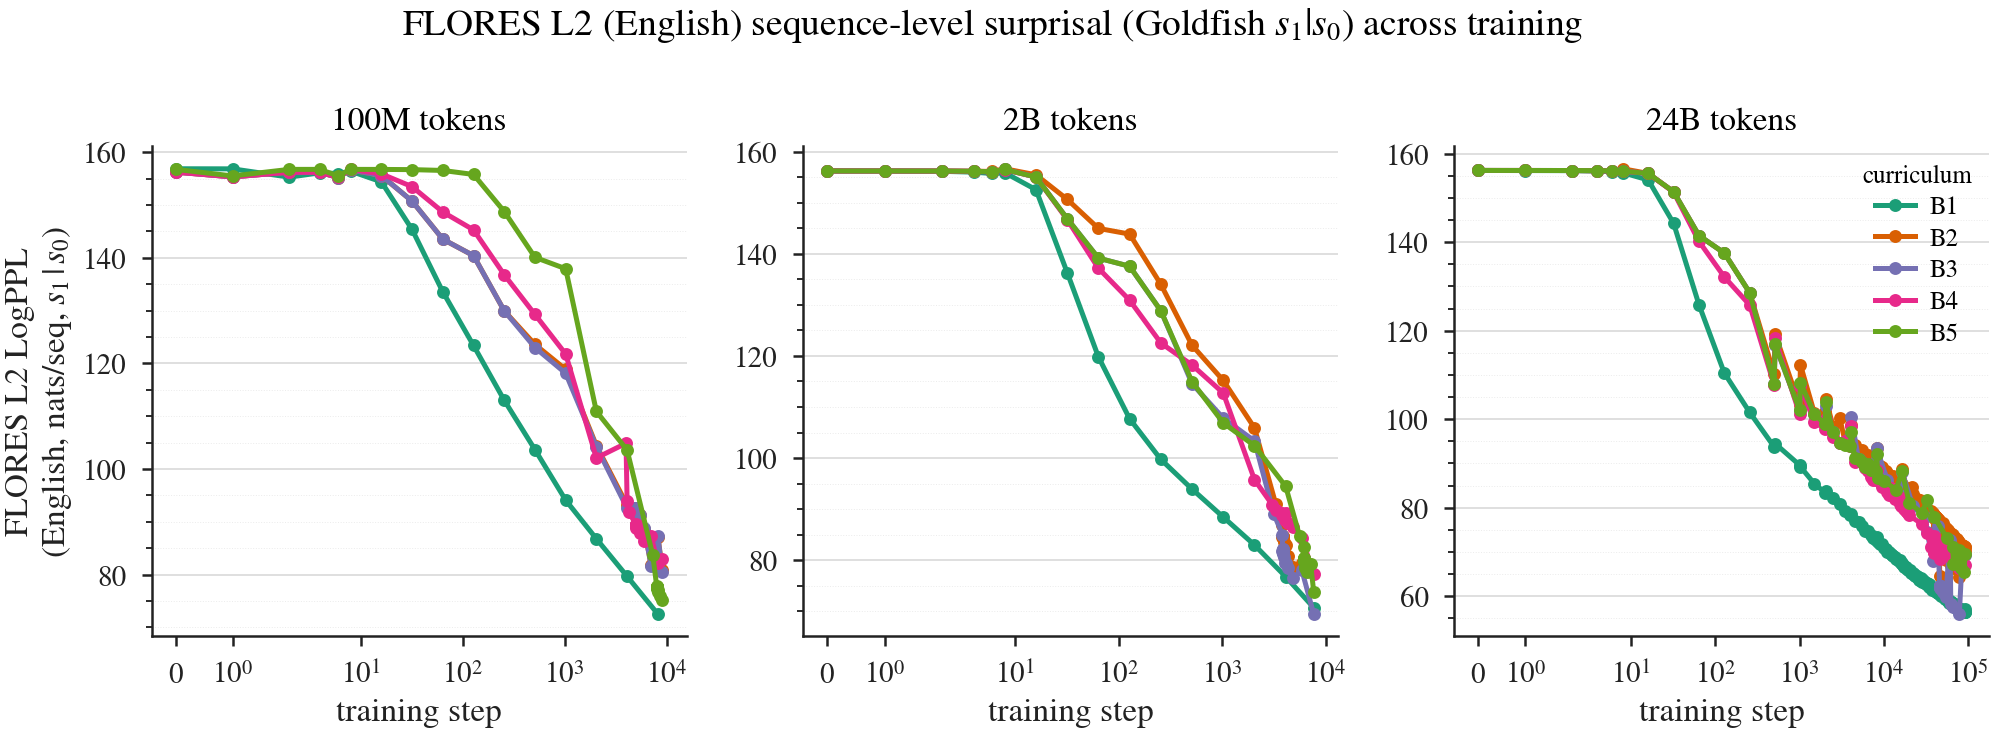
\includegraphics[width=\linewidth]{fig/flores/beetle-flores-l2.png}
%     \caption{FLORES sequence-level surprisal (LogPPL of $s_1\mid s_0$) across exposure curricula over training, at 100M/2B/24B token budgets. Top: L1. Bottom: L2. \textcolor{red}{something seems very wrong here. which language(s) is this for?} \textcolor{red}{let's not log scale the x axis. add vertical dashed lines for the L2 introduction for each curriculum}}
%     \label{fig:flores_curves}
% \end{figure}

% \textcolor{red}{for the next version of the paper, we can add extra experiments for EWC and TISO}




%\begin{itemize}
%    \item what is the effect of the curricula?
%    \item what is the effect of dataset size? and web data vs. babybabel?
%    \item comparing with EWC
%    \item comparing with monolingual and massively multilingual baselines
%\end{itemize}



% \textbf{JFLEG} \citep{napoles-etal-2017-jfleg} measures grammatical correction via learner-vs-corrected log-probability margins. 




%(RP$@0$: 62.09--56.64)
%, which suggests that different curricula might be better suited for different modelling objectives. % We do not further interpret this discrepancy beyond reporting ranking differences across metrics.

%JFLEG shows smaller and L1-dependent differences across curricula, with stronger effects in Germanic transfer settings (App.~\ref{appcomp:peda}, Tab.~\ref{tab:headline_pedagogical}).\footnote{An exploratory SAE-based analysis (App.~\ref{sec:meco-mech-app}) examines feature-level ablations. These results are reported as diagnostic only and are not used to support claims about underlying mechanisms.}




%In pedagogical evaluations (App.~\ref{appcomp:peda}, Tab.~\ref{tab:headline_pedagogical}), B1 performs best on cloze and CEFR-style metrics, while staged curricula perform better on MECO. These results are reported as task-dependent differences in ranking across evaluation settings. 

%\section{L2 Discrimination \& CEFR}\label{sec:discrimination}

%We next ask whether the curriculum effect carries over to grammatical discrimination.



%\textbf{BLiSS} \citep{gao2025bliss} scores bits-per-token preference margins over (good, learner-error, artificial-error) triplets via RP$@\tau$, NGS, and CPS, L1-stratified to separate matched- from mismatched-L1 transfer. 

%\textbf{JFLEG} \citep{napoles-etal-2017-jfleg} measures grammatical correction via learner-vs-corrected log-probability margins. \textbf{BLiSS:} staged curricula (B2/B3-33/B5) again exceed B1, but by a much smaller margin than on MECO. The FineWeb nld--eng order is B3-33 $>$ B5 $>$ B2 $>$ B4 $>$ B1 (RP$@0$: 62.09, 60.27, 60.05, 58.57, 56.64)---a spread of ${\sim}5$ points, against the ${\sim}78$-$\Delta\log L$ MECO spread. The best schedule is L1-dependent in the same way as MECO: B3-33 leads the Germanic cells, while B5 leads the Chinese cell (zho--eng HumanScale, RP$@0=64.25$, also the Chinese MECO leader). \textbf{JFLEG:} gains are modest and L1-dependent, strongest in Germanic transfer settings (per-cell figures in App.~\ref{appcomp:peda}); a targeted SAE-based ablation linking JFLEG correction behaviour to context-associated features is reported as an exploratory diagnostic in App.~\ref{sec:meco-mech-app}.

%Two patterns hold across tasks. First, the curriculum effect is much larger on incremental reading-time prediction (MECO) than on categorical grammatical discrimination (BLiSS/JFLEG): a schedule that sharpens short-horizon prediction can move graded reading-time fit substantially while moving categorical preference margins little, consistent with the much smaller BLiSS spread. Second, the best schedule is set by the L1 rather than the task (B3-33 for Germanic, B5 for Chinese). No single schedule is uniformly optimal, and the practical takeaway is to pick the schedule by L1 and target task. On pooled-L1 evaluation, the multilingual-LLM cohort (Gemma-2, Llama-3.1, Qwen-3) reaches RP$@0\approx66$--$71$, above every \beetle{} cell, so the BLiSS comparison is restricted to within-\beetle{} rankings. The same task-dependence extends to pedagogical probes (App.~\ref{appcomp:peda}, Tab.~\ref{tab:headline_pedagogical}): balanced exposure (B1) leads on closed- and open-cloze (CLOTH, Cambridge), JFLEG fluency, and the CEFR perplexity gradient, even as staged curricula lead on reading-time alignment---a prediction-vs-pedagogy trade-off rather than a uniform ranking. The within-\beetle{} BLiSS-vs-MECO trade-off itself (the two metrics order the curricula oppositely) is quantified in App.~\ref{appcomp:bliss}.

%Next, we evaluate whether our models function as reliable psycholinguistic instruments at lexical and sentence level. We treat the four benchmarks as partially dissociable signals (cf.\ App.~\ref{sec:pico-q2}) and follow appendix notation throughout (BLiSS RP$@0$, MECO $\Delta\log L$). \textbf{BLiSS} \citep{gao2025bliss} evaluates preference margins over (good, learner-error, artificial-error) triplets via NGS, CPS, and RP$@\tau$; data are L1-stratified to separate matched- from mismatched-L1 transfer. \textbf{CUP\&A5} \citep{mullooly2023cupa5} is a CEFR-stratified 200-item multiple-choice benchmark, evaluated following \citet{benedetto-etal-2024-using} via accuracy monotonicity across CEFR levels. \textbf{CLOTH} \citep{xie-etal-2018-cloth} is a B1--C1 cloze comprehension task. \textbf{JFLEG} \citep{napoles-etal-2017-jfleg} evaluates grammatical correction via learner-vs-corrected bits-per-token margins. \textbf{RC-MCQ} and \textbf{RACE} \citep{lai-etal-2017-race} serve as scale-limit controls (\S\ref{sec:discrim-cefr}).

%\paragraph{Method.} \textbf{BLiSS} \citep{gao2025bliss} scores bits-per-token margins on (good, learner-error, artificial-error) triplets via the Normalised Gap Score (NGS), the Correct-Preferred Sanity check (CPS), and the Random-Preference rate at threshold $\tau$ (RP$@\tau$); triplets are L1-stratified, separating matched- from mismatched-L1 transfer. We report NGS, CPS, and RP$@0$ per  \beetle \texttt{curricula} $\times$ \texttt{scale} $\times$ $\texttt{L1}$.  CUP\&A5 scores each checkpoint via CEFR-conditioned log-likelihood with argmax prediction, summarised by a monotonicity score $M = \rho(\mathbf{acc}, \mathbf{ideal}) - \sum_{i=1}^{4} \max(0, \mathrm{acc}_i - \mathrm{acc}_{i+1})$, where $\rho$ is Spearman correlation with the CEFR ordering and the penalty discourages non-monotone level transitions. CLOTH is reported as accuracy; JFLEG as the learner-vs-corrected log-probability margin.




%We evaluate on NLP grammatical tasks, reading time prediction, and L2 learning error prediction.  Across these evaluations, small exposure-controlled bilingual LMs can match or exceed substantially larger massively multilingual systems on cognitive tasks. But the optimal exposure curricula are task-specific:  sequential and late-onset schedules better predict L2 reading time; while balanced and simultaneous schedules dominate BLiSS error discrimination and CEFR-graded simulation.  Principled bilingual training setups may therefore provide stronger cognitive models of human psycholinguistic and acquisition.


%Through these evaluations, we have shown that
%\begin{itemize}
%    \item the curricula work - we see different behaviors
%    \item we closing the gap between open-data and closed-data models for cognitive modeling and modeling l2 behavior
%language processing
 %   \item the models also can help reduce WEIRD bias in cogsci/psycholinguistics (damian blasi, asifa majid (sp?)) %Bylund, E. (2022). 10 WEIRD Psycholinguistics. Struggles for Multilingualism and Linguistic Citizenship, 173.
%\end{itemize}

% Across MECO L2 reading-time alignment and BLiSS/JFLEG error discrimination, we observe a consistent dissociation in curriculum ordering. Human-inspired staged exposure schedules (B2/B3-33/B5) yield stronger alignment with L2 reading-time behaviour than balanced bilingual exposure (B1), particularly in early eye-movement measures (first-fixation, first-pass, spillover) and at smaller training scales where predictive competence is still developing. In contrast, BLiSS and CEFR-graded evaluations show a reversed pattern, with balanced or simultaneous curricula generally achieving stronger grammatical error discrimination, while staged schedules are narrower or weaker. This inversion is not explained by perplexity differences alone—iso-perplexity matching is directionally consistent but underpowered—and remains stable under hierarchical pooling and replication, indicating a task-dependent separation rather than a single globally optimal curriculum.

% We interpret this as a unified trade-off between incremental, L2-like predictive processing and longer-horizon grammatical discrimination. Staged exposure shifts probability mass toward earlier lexical access and reduces reliance on long-range contextual integration, improving MECO-style reading-time prediction while degrading sensitivity to extended grammatical dependencies required by BLiSS/JFLEG. The strength of this effect is scale-dependent, being most pronounced at smaller training budgets and diminishing as models acquire broader general predictive competence. Rather than implying a universal training prescription, these results highlight the utility of controllable exposure structure as an experimental axis: the \beetle{} framework  enables systematic manipulation of bilingual curriculum timing while holding architecture, tokenizer, and data fixed, providing a reusable substrate for probing how exposure dynamics shape L2-like processing and grammatical competence in neural language systems.


% \begin{itemize}
%     % \item future work/other options: trilingual and beyond
%     \item WEIRD bias in cogsci (damian blasi, asifa majid (sp?))
% \end{itemize}


%\textcolor{red}{[catherine: I think the discussion should only have 2 short-ish paragraphs summarizing the reading time and BLISS/JFLEG results. in the grand scheme of things, the main focus isnt about the specifics of Dutch vs. Chinese. i think it would be better to spend more of the discussion pitching the utility of these models and the training framework.] \textcolor{red}{[also, we should definitely report the number of models we're releasing, i think that number will be really impressive.]}}

%In this paper, we examined whether the temporal structure of bilingual exposure affects how well language models capture human L2 processing. Holding architecture, tokenizer, training data, and token budget constant allowed us to isolate exposure curriculum as the primary experimental variable. Across MECO L2 reading-time evaluations, staged curricula (B2/B3/B5) generally produced stronger alignment with human reading behaviour than balanced bilingual exposure (B1), particularly for Dutch and German L1 readers and at smaller training scales (App.~\ref{sec:meco-results}). The effect remained directionally stable under hierarchical pooling and seed replication, although differences among the staged curricula themselves were often small relative to variance (App.~\ref{sec:hier-model}; App.~\ref{sec:sig-robustness}).

%The central empirical result is that exposure timing influences psycholinguistic alignment independently of standard language-model quality metrics. Models trained with balanced bilingual exposure from the beginning of training were typically less predictive of human L2 reading times than models that first underwent an L1-dominant phase before English exposure. At the same time, staged curricula did not consistently improve perplexity or downstream grammatical evaluations (App.~\ref{sec:downstream}). In our experiments, behavioural alignment and conventional LM metrics therefore captured partially different properties of bilingual models.

%Reading-time analyses suggest that curriculum effects may be concentrated in earlier stages of incremental processing, with staged curricula showing somewhat stronger differences in first-pass and spillover measures associated with lexical access and immediate integration, weaker or less consistent effects for later integration-sensitive measures, and reduced long-context reliance in likelihood-decomposition analyses, although the observed differences in long-context reliance and layerwise encoding depth remain descriptive correlates of curriculum structure rather than demonstrated mechanisms (App.~\ref{sec:meco-stage-app}; App.~\ref{sec:meco-mech-app}; Tab.~\ref{tab:sig_decomp_curriculum}).

%The curriculum effect was not uniform across language pairs. Dutch and German readers showed relatively stable staged-over-balanced advantages across scales, whereas Chinese readers showed weaker and less consistent ordering. Hierarchical analyses likewise attributed a substantial portion of variance to L1 and residual factors, with curriculum contributing a smaller but consistently positive component (App.~\ref{sec:hier-model}; Tab.~\ref{tab:hier-varcomp}). These results suggest that the benefit of staged exposure depends partly on transfer structure between languages rather than functioning as a universal optimisation strategy.

%Scale moderated the curriculum effect in a similar way. The staged-over-balanced advantage was strongest at HumanScale-100M, weakened substantially at 2B tokens, and partially re-emerged at 24B (App.~\ref{sec:hier-model}; Tab.~\ref{tab:hier-contrasts}). This pattern suggests that exposure order matters most under constrained optimisation regimes, while larger-scale training partially reduces curriculum-dependent differences. Nevertheless, under matched sum-of-subwords aggregation, relatively small staged bilingual models remained competitive with substantially larger multilingual LLM baselines on MECO alignment (App.~\ref{sec:meco-baselines-app}). Because these systems differ in architecture, tokenizer, and training data, we treat this comparison as contextual rather than a controlled ranking.

%The contrast between MECO and BLiSS/JFLEG evaluations further indicates that different bilingual benchmarks reward different behavioural properties. Reading-time prediction consistently favoured staged curricula, whereas grammatical discrimination and learner-error benchmarks showed smaller or less stable differences, with some metrics favouring balanced exposure instead (App.~\ref{sec:downstream}). The negative correlation between BLiSS and MECO rankings (App.~\ref{appcomp:bliss}) suggests that these evaluations capture partially distinct dimensions of bilingual competence: MECO emphasises incremental predictive processing during comprehension, while BLiSS and pedagogical tasks place greater weight on explicit grammatical discrimination and learner-error sensitivity.

%The MECO experiments cover only a limited set of L1 populations, and many curriculum conditions rely on single-seed estimates (App.~\ref{sec:significance-comprehensive}). Although replicated analyses reproduced the overall staged-over-balanced trend, fine-grained ordering among staged curricula was not always stable across seeds (App.~\ref{sec:sig-robustness}). However, \beetle{} allows straightforward extension of pretraining experiments that allow a straightforward addition of more language pairs, bilingual/L2/multilingual learner settings. Further longitudinal learner benchmarks may help clarify which forms of exposure structure most strongly support human-like bilingual language processing in neural systems.



%The results position bilingual exposure scheduling as a central determinant of psychometric alignment in L2 language models, distinct from scale or conventional language-model quality alone. Across MECO reading-time prediction and BLiSS grammatical discrimination, staged curricula (B2/B3-33/B5) form a stable high-performing regime, while balanced exposure (B1) is consistently weaker on the principal psychometric readouts despite often achieving lower FLORES perplexity and reduced catastrophic forgetting. The clearest evidence comes from the matched Dutch-reader MECO comparisons, where staged \beetle{} curricula substantially outperform both multilingual LLM baselines and the closest prior bilingual setup, B-GPT \citep{arnett-etal-2025-acquisition}. At the same time, the curriculum ordering differs across evaluation axes: B2 tends to maximise MECO alignment whereas B3-33 more consistently maximises BLiSS preference separation, and the margins within the top-performing cluster remain relatively small under single-seed evaluation. We therefore interpret the curriculum effect as evidence for distinct bilingual representational regimes rather than for a single globally optimal training schedule. More broadly, the results suggest that psychometric predictive power depends not only on raw predictive accuracy, but on the structure of the predictive distribution learned during bilingual exposure. Prior L1 work has generally found that lower perplexity models exhibit stronger psychometric alignment with human reading behaviour, a trend termed the \emph{Quality--Power relationship} \citep{wilcox-etal-2023-language}. In the present bilingual setting, however, the relationship appears partially inverted: the lowest-perplexity bilingual curriculum (B1) is also consistently the weakest on MECO, while higher-perplexity staged curricula achieve substantially stronger reading-time alignment. We therefore interpret the proposed inversion conservatively as an observational pattern suggesting that the forms of predictive structure supporting multilingual robustness or retention are not necessarily the same as those supporting human-like L2 processing. The MECO analyses further suggest that curriculum structure primarily alters early lexical-access dynamics rather than later integrative processing. Relative to balanced exposure, staged curricula concentrate surprisal effects at lag~0, meaning that the predictive contribution of surprisal is strongest for the currently fixated word rather than for delayed spillover positions in subsequent words. Correspondingly, staged curricula improve first-pass reading-time prediction and redistribute predictive mass toward unigram and short-context components, while balanced exposure retains a larger contribution from longer-context representations distributed across later lags. In practical terms, the staged schedules rely more heavily on immediately available lexical expectations and short-range dependencies, whereas balanced exposure preserves broader contextual integration over longer horizons. The layerwise analyses are consistent with this interpretation: curriculum differences emerge most strongly in mid-to-late transformer layers, where balanced exposure shows greater alignment with contextual representations while staged schedules preferentially strengthen lexical and local-context signals. These findings resemble several established properties of human L2 reading, including stronger reliance on local lexical cues and weaker long-range predictive integration relative to L1 processing. Importantly, however, the present results do not imply that the models instantiate human cognitive mechanisms directly. The parallels are behavioural and representational rather than process-identical, and the mechanistic analyses remain limited in scope. The typological gradient further constrains the interpretation. Curriculum effects are strongest for Dutch and German readers and substantially attenuated for Chinese readers across both MECO and grammatical evaluations, suggesting that staged exposure interacts with transfer compatibility between L1 and L2 rather than functioning as a universally optimal bilingual strategy. Consistent with this interpretation, BLOOM retains an advantage on Chinese-reader MECO despite being substantially weaker than staged \beetle{} curricula in typologically closer Germanic conditions. The grammatical and mechanistic evaluations provide convergent, though necessarily limited, support for this interpretation of curriculum-induced representational restructuring. BLiSS and JFLEG indicate that exposure scheduling affects grammatical sensitivity beyond reading-time prediction, although the effects are weaker and more transfer-dependent than the MECO results. In JFLEG, SAE-based ablations targeting context-associated features identified through the context-share decomposition produce substantially larger degradations in grammatical-correction margins than matched frequency-based controls, suggesting that the decomposition captures functionally relevant distinctions between lexical and contextual predictive structure. We treat these analyses conservatively as diagnostic evidence rather than definitive causal demonstrations, since they are restricted to individual models, layers, and tasks. More broadly, the results suggest that exposure structure may matter as much as scale for certain forms of psychometric alignment. Structured \beetle{} bilinguals consistently outperform substantially larger multilingual LLMs on MECO, and staged curricula exceed the BLOOM-7b1 alignment threshold well before 200M tokens while maintaining the advantage across scale. The apparent transition around 2B tokens is therefore better characterised as a curriculum-sensitive crossover than as a uniform psychometric ceiling. Taken together, these findings position \beetle{} less as a single bilingual model family than as a controlled framework for studying how bilingual exposure schedules shape linguistic, psychometric, and representational behaviour across scales, language pairs, and transfer conditions..


%encoder--decoder, GPT-NeoX-style, and adapter-only alternatives, including BeetleMoE and BeetleSSM ), described in App.~\ref{sec:beetle-architecture-registry}\Future work could explore whether other architectures better model human bilingual language processing.




% \textcolor{red}{Data research. We will release infinigrams for each datasets, enabling better understanding of the data used to train the models. ask questions about generalization and contamination.}


%\paragraph{Continual learning.} 
%Reported experiments use EWC at language transitions \citep{kirkpatrick2017overcoming}, LAMOL-style generative replay, and a learning-rate plasticity boost at L2 onset. 

%\textcolor{red}{don't worry about reporting results, just pretend you haven't trained models. we can maybe add an appendix about this in the camera ready version.}



% \section{Conclusion}\label{sec:conclusion}


% \newpage 



% \newpage 



%\paragraph{Statistical Significance Testing} A limited seed sweep (${13, 42, 97}$) for nld-eng Human-Scale B1--B3 models shows moderate variance in auxiliary metrics, but variability within a curriculum family is substantially smaller than the differences observed between Beetle and BLOOM, which remain large in absolute terms. We plan to investigate per-seed $\Delta\log L$ results. We report standard inferential statistics, including paired bootstrap tests, permutation tests with Holm--Bonferroni correction against BLOOM, and effect sizes (Cohen’s $d_z$). In some cases, effect sizes appear large despite very small absolute differences in correlation values. This occurs because the underlying standard errors are extremely small at large sample sizes, making $d_z$ sensitive even when raw differences are minor. For this reason, we report raw correlation values alongside effect sizes and encourage interpretation based on both. We apply multiple-comparison corrections within logically coherent families of tests but do not correct across unrelated hypothesis groups (e.g., curriculum ranking vs. cross-model comparison), as these address distinct questions. 




%\begin{figure}[!ht]
 % \centering
  \includegraphics[width=\linewidth]%{fig/fig_best_bliss_vs_baselines.pdf}
%  \caption{\textbf{BLiSS results.} The best matched-L1 \beetle{} configuration is B5 zho--eng HumanScale (RP$@0=64.25$, NGS$=61.88$, CPS$=36.41$). For matched nld--eng, B3-33 leads (RP$@0=62.09$, NGS$=58.11$). Multilingual LLMs (Gemma-2, Llama-3.1, Qwen-3) reach RP$@0 \approx 66$--$71$ on pooled-L1 evaluation, exceeding all \beetle{} cells; comparisons are therefore restricted to within-\beetle{} rankings. \textcolor{red}{[catherine: i think it would be better to just do the same models from figure 3 and then also include the monolingual baseline.]}}
%  \label{fig:bliss_best}
%\end{figure}

%\paragraph{Key finding: stable high-performing regime under metric-dependent ordering.}  Across BLiSS, structured curricula (B2, B3-33, B5) again form a consistent high-performing regime, but with a different internal ordering than MECO. In particular, B3-33 tends to maximise preference separation (RP$@0$), while B2 and B5 remain competitive but are not consistently dominant across L1s. Balanced exposure (B1) is systematically weaker, indicating that exposure structure affects grammatical error discrimination even when controlling for scale.  We complement this with JFLEG, which measures grammatical correction ability via log-probability margins between learner and corrected sentences. Unlike BLiSS, which probes preference geometry, JFLEG reflects repair-oriented grammatical competence. Here, improvements under staged curricula are more modest and L1-dependent: gains are strongest in Germanic L1 transfer settings and attenuate under typologically distant transfer. Taken together, BLiSS and JFLEG suggest that exposure structure shapes grammatical sensitivity, but this effect is less uniform than the robust curriculum signal observed in MECO reading-time alignment.  In JFLEG, we use grammatical correction likelihoods to test whether ablating context-associated components identified in our decomposition disproportionately degrades error-correction performance relative to frequency-matched lexical controls, providing a limited causal validation of the proposed lexical–contextual separation. To examine whether the context-share decomposition generalises beyond reading-time prediction and preference-based discrimination, we perform a targeted SAE-based ablation analysis on grammatical correction behaviour. We train a sparse autoencoder on a fixed hidden layer to obtain a feature dictionary over activations, and identify features most strongly associated with the context-share signal induced by our decomposition. We then ablate the top-50 such features at inference time and compare the resulting change in JFLEG learner–corrected fluency margins against a frequency-matched control set of SAE features selected using the same procedure but aligned to unigram surprisal components. We observe a larger reduction in JFLEG margins under ablation of context-share–associated features than under the matched frequency control (approximately 1.9×–6.7× across conditions). We interpret this as indicating that the SAE-derived context-share subspace is more closely aligned with grammatical correction behaviour than frequency-related features, though the analysis remains limited to a single model, layer, and task Across BLiSS and MECO, \beetle{} curricula form a stable high-performing regime in matched L1--L2 settings, but with metric-dependent internal ordering. In particular, the B2, B3-33, and B5 configurations consistently occupy the top tier on both BLiSS (RP$@0$) and MECO ($\Delta\log L$), while differing in rank across metrics (e.g.\ B2 highest on MECO, B3-33 highest on BLiSS). The magnitude of separation within this cluster is small (approximately $\sim$2 BLiSS points and $\sim$20 MECO units), yet sufficient to produce rank reversals across evaluation axes. Balanced exposure (B1) is consistently lower on BLiSS (approximately 5--6 points below the top cluster) and shows modest but non-degenerate differences on MultiBLiMP. \paragraph{BLiSS curriculum-by-task observation}\label{sec:discrim-bliss} Within \beetle{}, FineWeb nld--eng ordering is B3-33 $>$ B5 $>$ B2 $>$ B4 $>$ B1 (RP$@0$: 62.09, 60.27, 60.05, 58.57, 56.64). On zho--eng HumanScale, B5 reaches 64.25, the highest observed value (Fig.~\ref{fig:bliss_best}). The top three curricula form a narrow band (within $\sim$2 points) and are not separable under single-seed evaluation, suggesting a shared regime of performance rather than strict ordering stability. 



%for next version of the paper-
% \textcolor{red}{We also compare to EWC, which was proposed in \citet{constantinescu2025InvestigatingCriticalPeriod} (ADD FIGURE). We find that }



% \textcolor{red}{is this true?}
% \textcolor{red}{Effect of more training data – unclear to me; better for Dutch 24B, similar for German/Dutch}. 


% EuroLLM-1.7B and 9B \citep{martins2024eurollm}, , Gemma-2-2B and 9B \citep{team2024gemma}, Qwen-3-4B and 8B \citep{bai2023qwen,yang2025qwen3}, Llama-3.1-8B \citep{touvron2023llama, grattafiori2024llama}, Baichuan-7B \citep{yang2023baichuan}, Yi-6B \citep{young2024yi}, BLOOM-560m, 1.1B, 1.7B, 3B, and 7.1B \citep{workshop2022bloom}, and , reported for continuity with prior L2LM literature. For MECO~L2 we additionally compare against the mBERT pseudo-surprisal baseline of \citet{de-varda-marelli-2022-effects}. \textcolor{red}{update this when we finalize models.}

%\textcolor{red}{[Specify coverage: are these available for every dataset size and every dataset, or only a subset?]}



%Bilingual language models (LMs) provide a controlled setting for studying how training conditions shape second-language (L2) behaviour, but prior work often varies exposure structure, scale, and architecture simultaneously, making attribution difficult. We introduce \beetle, a controlled bilingual pretraining framework that standardises architecture, tokeniser, target language, and training budget across conditions, enabling comparisons across exposure curricula under a unified training pipeline. We train bilingual LMs under multiple exposure schedules and L1s, and evaluate them on human L2 reading-time prediction and grammaticality judgment tasks. Staged exposure curricula align better with human reading times than balanced bilingual exposure, particularly at smaller training scales and for closely related language pairs, with the direction of effects consistent across seeds though absolute magnitudes vary. Exposure effects are task- and L1-dependent, substantially weaker on grammaticality judgment and not consistently associated with lower language-model perplexity. Results suggest that bilingual exposure schedules shape behavioural alignment independently of perplexity within a controlled training framework.

%Bilingual language models (LMs) provide a controlled and tractable testbed for studying second-language (L2) acquisition, yet prior work has not systematically disentangled the effects of exposure \emph{structure} and training \emph{scale}. Existing studies often vary curricula, language pairs, continual-learning settings, architectures, and data quantities simultaneously, obscuring the influence of each factor. We introduce \beetle, a modular bilingual pretraining and analysis framework for studying multilingual training and modelling human bilingual language processing. We use \beetle~ to pretrain bilingual LMs with fixed architecture, tokeniser, and L2 (English) while varying L1, training data scale, and exposure curricula for eight typologically diverse L1s. %These curricula include: balanced, simultaneous, sequential, classroom-style, and late-onset L2 exposure across
% We consider eight typologically diverse L1s targeting L2 English at both human- and web-scale data sizes. 
%Our results suggest smaller, exposure-controlled bilingual LMs can consistently outperform substantially larger massively multilingual LMs on both cognitive evaluations: the gap between our models and multilingual/bilingual LLMs exceeds 100~$\Delta\log L$ on the matched Dutch-reader condition. Compared with the closest matched bilingual prior, Beetle models achieve a 1.58$\times$ improvement in $\Delta$logL.  Principled bilingual training setups may provide stronger cognitive models of human psycholinguistic and acquisition behaviour.




%Experiments target L2 English, the only L2 with simultaneous coverage by population-scale eye-tracking (MECO~L2; \citealp{siegelman2025wave}), CEFR-stratified L2 error-discrimination data \citep{gao2025bliss}, and pre-tested CEFR-graded learner evaluation tasks  \citep{napoles-etal-2017-jfleg,mullooly2023cupa5}. We compare Beetle models to larger multilingual models, e.g. BLOOM \citep{workshop2022bloom}, XGLM, Apertus  \citep{swiss-ai-2025-apertus}, Llama \citep{touvron2023llama}, and Qwen \citep{bai2023qwen} (\S\ref{sec:comparator-landscape}) \textcolor{red}{[FIX REFERENCE]}, finding  exposure curricula in bilingual LM pretraining can surpass LLM L2 reading-time performance on tighter parameter budgets. Across learner proficiency tasks, structured \textcolor{red}{[catherine: instead of "structured", can we make a stronger connection between the curricula which were designed to be human-inspired? it's not just that they're structured, but that the curricula which we designed to be more similar to bilingual language experience leads to more human-like models} curricula consistently outperform balanced exposure, exhibiting stable but metric-dependent improvements in grammatical sensitivity and CEFR-aligned proficiency, while remaining less sharply separated than in reading-time–based evaluations. 


%Exposure curricula yield a  \textbf{1.58$\times$} $\Delta$logL reading time improvement on matched bilingual LMs \citep{arnett-etal-2025-acquisition}.   
%\textcolor{red}{[here we need 1-2 sentences summarizing BLISS/CEFR results]}
%But the optimal curriculum is task-specific: sequential and late-onset schedules better predict reading time; balanced and simultaneous schedules dominate BLiSS error discrimination and CEFR-graded pedagogical simulation.   Beetle's L2 reading time performance continue improving past 2B, suggesting the $\sim$2B-token inflection of \citet{aoyama-wilcox-2025-language} is curriculum-modulated.  


%---precisely what this paper addresses by introducing the largest bilingual L2 reading-time benchmark to date, spanning 13 languages and systematically varying exposure structure, and building on prior L2LM work along three dimensions: broader language coverage (13 typologically diverse languages), continuous exposure parameterisation replacing binary training regimes, and unified cognitive–pedagogical evaluation using MECO L2 reading times, BLiSS, and CEFR measures, while its continual-learning framework subsumes prior strategies such as EWC, MAML-style adaptation, and learning-rate modulation, and scales training on FineWeb (100M–24B tokens) to jointly analyse scaling, transfer, and psycholinguistic predictive power.

%as word length, frequency, and predictability, with lower-proficiency readers relying more on context-invariant cues than on predictive context \citep{berzak2023eye, nahatame2025relative}


% $-\log P(w_i \mid w_{<i})$. 
%Surprisal enters a regression alongside lexical covariates and is scored by the improvement in log-likelihood it yields over a frequency-and-length baseline ($\Delta\log L$; \citealp{wilcox2020predictive, wilcox-etal-2023-language, kaye2025sentence}). Psychometric predictive power therefore depends on how well a model's probability distribution aligns with human processing, not just on raw quality. The literature has explored LM alignment more extensively for L1 than for for L2 \citep{de-varda-marelli-2022-effects, aoyama2024modeling}. \textcolor{red}{[catherine: i would take the opportunity here to highlight that while this paper is closely related to these other papers, in the scheme of reading time modeling, bilingual data is really under-represented and this paper fix that.]} This paper builds on prior L2LM work along three dimensions: broader language coverage (13 languages), continuous exposure parameterisation replacing binary training regimes, and unified cognitive–pedagogical evaluation using MECO L2 reading times, BLiSS, and CEFR measures, while its continual-learning framework subsumes prior strategies such as EWC, MAML-style adaptation, and learning-rate modulation, and scales training on FineWeb (100M--24B tokens) to jointly analyse scaling, transfer, and psycholinguistic predictive power.


%\begin{table*}[!ht]
%\centering
%\begin{tabular}{@{}l l c c c l@{}}
%\toprule
%\textbf{ID} & \textbf{Curriculum} & \textbf{L2 onset} & \textbf{Final L1:L2} & %\textbf{Transition} & \textbf{Key manipulations} \\
%\midrule
%B1 & Balanced & step 0 & 50:50 & none &
%\small{50:50 from step~0; noise $\sigma{=}0.02$; LR warmup} \\
%B2 & Simultaneous & 50\% & 50:50 & sigmoid &
%L1 then ramp to 50:50 \\
%B3 & Sequential & 50\% & 33:67 & sigmoid &
%L1 then L2-dominant mixture \\
%B4 & Classroom & step 0 & 80:20 & \small{constant mean + bursts} &
%\small{constant 20\% L2 mean, bursty L2 episodes} \\
%B5 & Late & 80\% & 50:50 & sigmoid &
%\small{delayed L2; optional EWC} \\
%\bottomrule
%\end{tabular}
%\caption{\beetle{} exposure curricula B1--B5. Each curriculum fixes L2-onset timing, final L1:L2 ratio, and the transition shape between the L1-only and bilingual phases. }
%\label{tab:curricula-overview}
%\end{table*}



% Recent findings of systematic similarities in language-model behaviour across architectures, training data, and scale \citep{michaelov2025language} motivate the comparison of multiple backbones; the \beetle{} training library also implements encoder--decoder, GPT-NeoX-style, and adapter-only alternatives, including BeetleMoE and BeetleSSM ), described in App.~\ref{sec:beetle-architecture-registry}.
%(implemented but not evaluated in this paper
%\paragraph{Architecture.} The default backbone, \textbf{PicoDecoder} \citep{diehl-martinez-etal-2025-pico}, is a 125M-parameter LLaMA-style causal decoder \citep{touvron2023llama}: 14 layers, $d_{\mathrm{model}}=768$, 12 attention heads with one KV head (grouped-query attention), Rotary Position Embeddings, SwiGLU activations, RMSNorm, 50K BPE vocabulary, sequence length 512. \textcolor{red}{[catherine: we could highlight that this architecture is more modern than a lot of the other related work (esp. mine).]}PicoDecoder's compatibility with Pico-Analyze \citep{diehl-martinez-etal-2025-pico}, which allows \beetle{} models to mechanistically analyse how bilingual pretraining manipulations affect weight geometry (e.g., shifts in effective rank or representational similarity) across checkpoints \citep{diehl-martinez-etal-2025-pico,inaba-etal-2025-bilingual} (App.~\ref{sec:beetle-analyze}). The \beetle{} training library also implements other architectures, which we describe in App.~\ref{sec:beetle-architecture-registry}. \textcolor{red}{[catherine: might be interesting to make a connection to James's neurips paper last year about similarities across architectures to motivate comparing across architectures. ]}


%\textcolor{red}{what kind of tokenizer is default (what training framework)? what are the other options?}


%; models gradual early bilingual acquisition with increasing L2 exposure.



%\begin{itemize}\setlength\itemsep{-1pt}
%\item \textbf{B1 Balanced.} constant 50:50 ratio from step~0, representing full bilingual exposure.
%\item \textbf{B2 Simultaneous.} L1-only for the first 50\% of training, then sigmoid-ramp to 50:50, representing late-onset simultaneous bilingual exposure.
%\item \textbf{B3 Sequential.} L1-only for 50\% of training, then sigmoid-ramp to an L2-dominant 33:67 mix. 
%\item \textbf{B4 Classroom.} Constant 20\% L2 mean from step 0 with bursty L2 episodes around that mean (no staged transition) --- the temporal-structure diagnostic. B4 is matched in stationarity-of-mean to B1 and matched in imbalance to B3/B5, isolating timing from proportion. B4 models are trained without EWC to enable comparison with B2 (temporal-structure-vs-proportion contrast.
%\item \textbf{B5 Late.} L1-only for 80\% of training, then sigmoid-ramp to 50:50 --- late-onset L2 immersion.
%\end{itemize}


%\textcolor{red}{i think there was other information here that should be added back - tokenizer training, how flexible is it wrt to data mixtures/which dataset you use. other features of the training framework?}



% ---------------------------------------------------------------------
%  Wide 10-column table: must stay full-width (table*).  Right-aligned
%  numeric columns; \footnotesize.
% ---------------------------------------------------------------------
% \begin{table*}[H]
%   \centering
%   \footnotesize
%   \setlength{\tabcolsep}{4.5pt}
%   \caption{\textbf{Per-L1 matched MECO reading-time alignment
%   ($\Delta\log L$): full numeric data behind
%   Fig.~\ref{fig:meco-typ-l1-staged-balanced}.} Each matched per-L1
%   bilingual \beetle{} curriculum (B1 balanced, B2 simultaneous, B3-33
%   sequential; 125M params) evaluated on its own L1's MECO L2 readers at
%   two pretraining scales (FineWeb-100M, FineWeb-2B), every multilingual
%   LLM (by model; $n{=}22$, evaluated on all cohorts), the LLM box-summary
%   statistics that the orange boxes in
%   Fig.~\ref{fig:meco-typ-l1-staged-balanced} draw, and the
%   monolingual-English HumanScale anchor (dashed line). LLM and
%   monolingual baselines are scale-independent (identical across panels).
%   Columns are the eight MECO reader cohorts, by ISO~639-3 L1 code,
%   ordered by approximate typological distance to English: nld~Dutch,
%   deu~German, ita~Italian, rus~Russian, hin~Hindi, tur~Turkish,
%   eus~Basque, zho~Chinese. $\Delta\log L$ is comparable only \emph{within}
%   a column (same readers), so cross-cohort magnitudes reflect cohort
%   size, not effect size. \textbf{Bold} = best model per column (across all
%   \beetle{} and LLM rows).}
%   \label{tab:meco_per_l1_matched}
%   \begin{tabular}{@{}llrrrrrrrr@{}}
%     \toprule
%     & & \multicolumn{8}{c}{MECO $\Delta\log L$ by L1 reader cohort (typ.\ distance to English $\rightarrow$)} \\
%     \cmidrule(lr){3-10}
%     Model & Params & nld & deu & ita & rus & hin & tur & eus & zho \\
%     \midrule
%     \multicolumn{10}{@{}l}{\emph{\beetle{} bilingual, FineWeb-100M}} \\
%     \quad B1 balanced & 125M & 32.2 & 101.5 & 42.0 & 132.3 & 102.6 & 31.8 & 65.6 & 132.9 \\
%     \quad B2 simultaneous & 125M & 37.2 & 175.8 & 70.2 & 253.5 & 48.7 & 69.3 & 91.0 & 124.2 \\
%     \quad B3-33 sequential & 125M & 37.3 & 172.3 & 61.8 & \textbf{267.1} & 50.5 & 68.4 & 90.7 & 135.4 \\
%     \addlinespace[2pt]
%     \multicolumn{10}{@{}l}{\emph{\beetle{} bilingual, FineWeb-2B}} \\
%     \quad B1 balanced & 125M & 30.6 & 85.4 & 34.7 & 188.8 & 98.8 & 45.1 & 63.6 & 155.6 \\
%     \quad B2 simultaneous & 125M & 35.5 & 85.9 & 43.2 & 136.2 & 38.9 & 33.6 & 88.1 & 149.0 \\
%     \quad B3-33 sequential & 125M & 40.2 & 100.8 & 43.3 & 162.8 & 90.5 & 41.3 & 89.7 & 133.5 \\
%     \midrule
%     \multicolumn{10}{@{}l}{\emph{Multilingual LLMs (by model)}} \\
%     \quad LLM-jp-3-150M & 150M & 46.4 & \textbf{207.8} & \textbf{106.3} & 201.4 & 200.5 & 43.6 & 99.7 & 154.1 \\
%     \quad LLM-jp-3-440M & 440M & 47.8 & 202.5 & 101.2 & 163.0 & \textbf{224.7} & 46.7 & \textbf{103.5} & \textbf{177.9} \\
%     \quad BLOOM-560M & 560M & 44.3 & 182.1 & 79.2 & 150.9 & 217.0 & 35.9 & 96.6 & 149.2 \\
%     \quad LLM-jp-3-980M & 980M & 31.8 & 151.8 & 73.6 & 106.5 & 172.7 & 29.1 & 69.3 & 125.3 \\
%     \quad BLOOM-1.1B & 1.1B & 41.1 & 184.5 & 91.6 & 153.1 & 222.7 & 41.7 & 87.6 & 164.2 \\
%     \quad BLOOM-1.7B & 1.7B & 34.8 & 150.3 & 82.1 & 135.0 & 189.5 & 36.5 & 77.0 & 137.0 \\
%     \quad EuroLLM-1.7B & 1.7B & 16.4 & 104.6 & 56.7 & 81.0 & 142.4 & 24.4 & 42.0 & 88.7 \\
%     \quad LLM-jp-3-1.8B & 1.8B & 24.3 & 127.9 & 75.0 & 73.7 & 160.8 & 28.1 & 55.1 & 97.0 \\
%     \quad Gemma-2-2B & 2B & 17.4 & 124.7 & 69.9 & 63.2 & 132.1 & 28.2 & 47.0 & 67.4 \\
%     \quad BLOOM-3B & 3B & 24.3 & 143.2 & 72.9 & 101.8 & 173.4 & 37.2 & 54.4 & 122.9 \\
%     \quad LLM-jp-3-3.7B & 3.7B & 20.7 & 116.7 & 63.9 & 55.8 & 151.8 & 21.1 & 45.7 & 80.8 \\
%     \quad Qwen3-4B & 4B & 16.4 & 121.2 & 58.6 & 60.4 & 140.9 & 23.3 & 51.0 & 76.4 \\
%     \quad XGLM-4.5B & 4.5B & 8.8 & 19.3 & 31.1 & 85.0 & 24.0 & 20.5 & 4.6 & 23.6 \\
%     \quad Yi-6B & 6B & 14.8 & 111.4 & 61.0 & 47.9 & 146.6 & 15.5 & 47.2 & 62.4 \\
%     \quad Baichuan-7B & 7B & \textbf{88.3} & 185.1 & 100.3 & 220.3 & 17.7 & \textbf{76.3} & 93.8 & 31.2 \\
%     \quad BLOOM-7.1B & 7.1B & 20.2 & 116.0 & 65.4 & 55.3 & 157.5 & 20.8 & 54.1 & 84.7 \\
%     \quad Apertus-8B & 8B & 15.5 & 116.2 & 61.4 & 57.9 & 119.6 & 23.8 & 38.0 & 62.7 \\
%     \quad Llama-3.1-8B & 8B & 12.2 & 97.9 & 45.3 & 47.3 & 123.8 & 14.4 & 30.8 & 55.3 \\
%     \quad Qwen3-8B & 8B & 12.7 & 107.9 & 55.6 & 48.1 & 126.1 & 17.8 & 36.2 & 55.6 \\
%     \quad EuroLLM-9B & 9B & 11.9 & 93.3 & 49.7 & 39.1 & 106.9 & 17.2 & 32.6 & 50.7 \\
%     \quad Gemma-2-9B & 9B & 8.5 & 97.8 & 51.1 & 38.8 & 103.1 & 17.9 & 32.2 & 50.4 \\
%     \quad LLM-jp-3-13B & 13B & 11.7 & 103.2 & 54.1 & 35.9 & 129.1 & 15.6 & 36.6 & 59.9 \\
%     \addlinespace[2pt]
%     \multicolumn{10}{@{}l}{\emph{LLM distribution (box summary)}} \\
%     \quad LLM max & --- & 88.3 & 207.8 & 106.3 & 220.3 & 224.7 & 76.3 & 103.5 & 177.9 \\
%     \quad LLM Q3 & --- & 34.1 & 151.5 & 78.1 & 127.9 & 173.2 & 36.3 & 75.1 & 124.7 \\
%     \quad LLM median & --- & 18.8 & 119.0 & 64.6 & 68.4 & 144.5 & 24.1 & 49.1 & 78.6 \\
%     \quad LLM Q1 & --- & 13.2 & 105.4 & 55.9 & 49.9 & 124.4 & 18.6 & 36.9 & 56.7 \\
%     \quad LLM min & --- & 8.5 & 19.3 & 31.1 & 35.9 & 17.7 & 14.4 & 4.6 & 23.6 \\
%     \midrule
%     Monolingual-English anchor & 125M & 64.8 & 72.1 & 27.5 & 129.5 & 46.8 & 10.3 & 83.9 & 51.5 \\
%     \bottomrule
%   \end{tabular}
% \end{table*}



\begin{table}[t]
\centering
\small
\setlength{\tabcolsep}{3pt}
\renewcommand{\arraystretch}{1.1}
\begin{tabular}{llccc}
\toprule
\textbf{$L_1$--$L_2$--$L_3$} & \textbf{Curr.} & \textbf{BLiMP} & \textbf{NL} & \textbf{Zho} \\
\midrule
eng--nld--zho & T1 bal.   & 58.1 & 66.2 & 64.5 \\
eng--nld--zho & T3 her.   & 58.8 & 61.3 & 62.0 \\
\midrule
nld--eng--zho & T1 bal.   & 55.7 & 67.8 & 65.1 \\
nld--eng--zho & T3 her.   & 53.1 & \textbf{71.9} & 61.6 \\
\midrule
zho--eng--nld & T1 bal.   & 57.7 & 65.3 & 66.2 \\
zho--eng--nld & T3 her.   & 53.5 & 60.5 & \textbf{70.0} \\
\bottomrule
\end{tabular}
\caption{\small Final-checkpoint grammaticality accuracy (\%) for trilingual \textsc{BeetleLM} models on \textsc{BabyBabel}. T1 uses balanced exposure; T3 uses heritage-dominant exposure with periodic re-exposure.}
\label{tab:trilingual_minimal}
\end{table}



%\begin{table*}[t!]
%\centering
% \tiny
%\begin{tabular}{@{}llllllll@{}}
%\toprule
 % & \multicolumn{9}{c}{\textbf{L1}}      \\ \midrule
 %  & \texttt{nld} & \texttt{deu} & \texttt{ita} & \texttt{rus} & \texttt{eus} & \texttt{hin} & \texttt{tur} \\ \cmidrule(l){2-8}
%\textbf{B1} & 63.9 & 63.6 & 62.7 & 60.9 & 62.1 & 63.8 & 61.1  \\
%\textbf{B2} & 57.6 & 52.8 & 53.7 & 53.7 & 52.6 & 54.6 & 53.3 \\
%\textbf{B3} & 57.4 & 54.8 & 54.3 & 53.4 & 54.0 & 55.0 & 53.3  \\
%\textbf{B4} & 58.4 & 57.1 & 56.1 & 55.9 & 56.0 & 57.3 & 54.2  \\
%\textbf{B5} & 62.8 & 62.7 & 61.6 & 60.0 & 60.7 & 62.1 & 61.0 \\ \bottomrule
%\end{tabular}
%\caption{\textcolor{red}{I don't think a table is the best way to visualize this. I think it would be nice to show this with bar plots maybe? each language can be a facet and each bar is a curriculum (keeep same color coding as figure 1.} }
%\label{tab:blimp-main}
%\end{table*}
